\chapter{Context}

\lettrine{D}{esign} process and robust optimization are major purposes of engineering works dealing with numerical simulations, especially in aeronautical or automotive industry~\cite{duchaine2009}. Despite the large amount of work that has been devoted to the design of efficient optimization techniques, the design process still requires important investments (financial and human)~\cite{forrester2009}. As a consequence, design errors appear after the industrialization phase and the implications these can have may be critical. A classical example of such failure is the Space Shuttle \emph{Challenger} disaster in 1986~\cite{draper1995}. During the Space Shuttle's ascent, a failure of O-ring seals on its right solid rocket booster caused its disintegration. It has been shown that an uncertainty on the behaviour of this O-ring had been a key factor to the accident. On the launch day, the temperature was particularly low and the effect of such low temperature on the O-ring was not known. Engineers had to extrapolate the response of the system to this event. Linked to a strong pressure at NASA for this launch, the decision to maintain the launch was made even-though engineers warned about the uncertainties of their findings. This lead to the creation of NASA's Safety, Reliability, Maintainability, and Quality Assurance (SRM\&QA) program.

Computational Fluid Dynamics (CFD) tools have been used more and more in the past decades to decrease the number of iterations between conception and experiments, and to avoid irreversible errors during the preliminary design phase. Nowadays, CFD codes have reached maturity and represent more accurately physical flow phenomena. Complex flow simulations on high-resolution grids are possible thanks to the continuous developments in numerical models and in High Performance Computing (HPC). Nevertheless, deterministic simulations only provide limited knowledge about a system. Uncertainties in the numerical model as well as in the problem formulation or inputs are necessarily present and translate into uncertainties in the outputs~\cite{Sacks1989}---see~\cref{fig:context}.

\begin{figure}[!h]
\centering
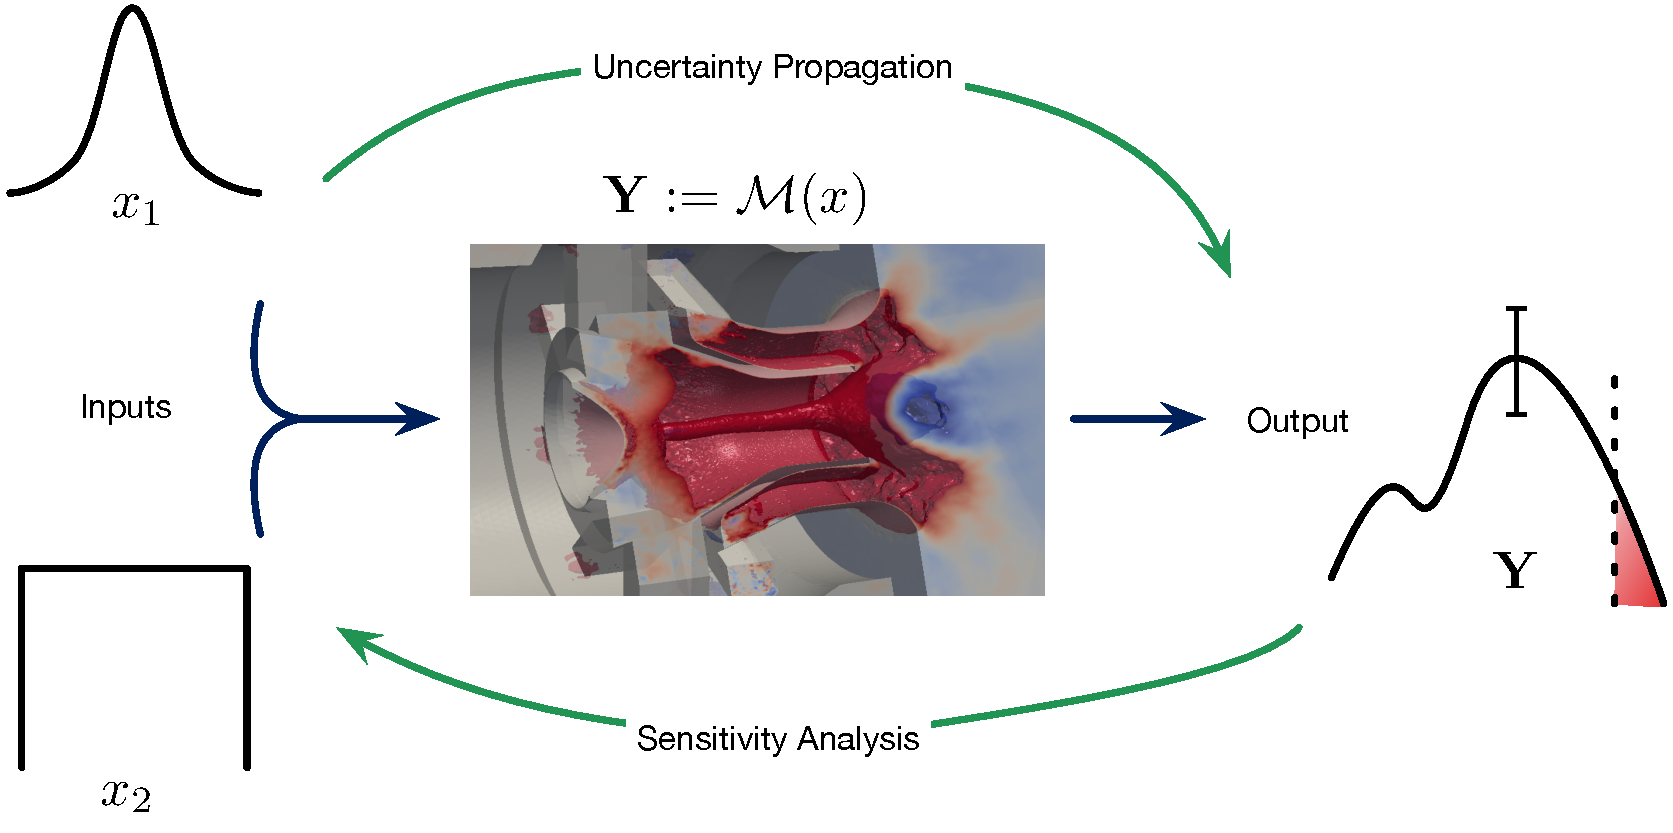
\includegraphics[width=\linewidth,keepaspectratio]{fig/literature/schema_UQ.pdf}
\caption{Schematisation of the Uncertainty Quantification procedure.}
\label{fig:context}
\end{figure}

The output variability of a system can be confusing regarding the source of these uncertainties. Does it come from our model or from the physics? Uncertainties can be classified as:

\begin{description}
	\item [Aleatoric:] intrinsic to our system,
	\item [Epistemic:] due to our lack of knowledge. We can reduce it by improving our model or adding experiments,
	\item [Numerical error:] due to the construction of our numerical scheme.
\end{description}

Ideally, our model should only contain aleatoric uncertainties as it is represents the physical variability of the system. However, the diversity of uncertainties due to the CFD boundary conditions or initial conditions as well as of model parameters (input data, geometry, simplification of the model physics, etc.) limits the predictivity of the simulations: the Quantity of Interest (QoI) can be easily affected and shadowed by the conjugation of all these types of uncertainties. This assessment explains why Uncertainty Quantification (UQ) is now becoming a mandatory step in application-oriented modelling for operational and industrial purposes~\cite{degennaro2015,masquelet2017}. It provides insight into the level of uncertainty in the numerical simulation results but also gives access to a Sensitivity Analysis (SA) which aims at describing the respective influences of the input parameters on the QoI. The inclusion of UQ in a design optimization cycle hence allows manufacturers to design quicker and obtain better, cheaper and more robust (i.e. more stable) products. Depending on the question we seek to answer, we have to determine the type of UQ study to conduce:

\begin{itemize}
	\item \emph{Uncertainty Propagation,}\hfill\\
Propagate an initial perturbation within the system and observe its outputs.
	\item \emph{Sensitivity Analysis,}\hfill\\
Rank the input parameters regarding their impact on the output.
	\item \emph{Risk assessment.}\hfill\\
Observe the probability to exceed a threshold or the probability of a particular quantile.
\end{itemize}

Each question is answered using specific tools and it special care has to be taken if ones want to conduce multiple analysis. It might not be possible to reuse the same data used for Uncertainty Propagation to do Sensitivity Analysis.

Classical UQ methods, based on the \emph{Monte-Carlo} approach, require a large number of simulations~\cite{saltelli2007}, which quickly go beyond the limits of available resources (CPU, financial costs). This is especially true when it comes to large dimensional problems, both with respect to the domain discretization and to the number of uncertain input parameters. The cost of the UQ study can, however, be significantly reduced when the experiment is replaced by a proxy, or surrogate model, which is formulated in a parameter space and which is fast to evaluate for any set of uncertain variables~\cite{martin2005}. 

\begin{quotation}

{\fontfamily{FiraCode-Light}\selectfont

%\textit{
The purpose of this thesis is to propose some directions of improvement on various methodological aspects of Uncertainty Quantification applied to costly numerical environments. The methods developed can be used in various fields and are demonstrated through multiple applications. Moreover, these methods are not limited to the use of numerical experiments and can be used equally for \emph{in vivo} experiments.
%}

}
\end{quotation}

\newpage

\section*{Organisation}
%\addcontentsline{toc}{section}{}

This manuscript is divided into four parts and is tailored as followed: 

\begin{description}
	\item[\Cref{part:intro}] \emph{after a general introduction about the context of this thesis,  \cref{chap:review} reviews the literature on concepts and methods around UQ,}\hfill\\
\Cref{sec:doe} goes from a state-of-the-art on the different methods to plan experiments; then \cref{sec:uq} describe the different technique commonly used to perform UQ as well as the latest advances. As explained above, such statistical analysis may require the usage of a surrogate model which are detailed in~\cref{sec:surrogate}. Once the uncertainties have been propagated, \cref{sec:visu} presents how uncertainties are visualized. After this literature review, some scientific questions arise and the complete scope of this thesis work is given in~\cref{chap:questions}.

	\item[\Cref{part:contributions}] \emph{presents my scientific contributions,}\hfill\\
In~\cref{chap:batman}, a new UQ open-source tool is introduced. It serves as a demonstrator for all the methods developed. Following, \cref{chap:doe,chap:resample,chap:visu}~are the responses to the scientific questions rose.

	\item[\Cref{part:applications}] \emph{some applications of the new methods are proposed through~\cref{chap:mascaret,chap:ls89,chap:swirler,chap:optim,chap:psaap},}\hfill\\

	\item[\Cref{part:conclusion}] \emph{put a point on this thesis work and draw some perspectives for futur work.}
\end{description}


\chapter{Literature Review}\label{chap:review}

\section{Design of Experiments}\label{sec:doe}

\lettrine{O}{ne} of the main objectives when performing numerical---or real---experiments is to understand the variation of a Quantity of Interest (QoI) with respect to the variation of some input parameters~\citep{Sacks1989}. Each experiment, or sample, corresponds to a particular set of input parameters $x_k$ with $k \in [1, \dots , d]$, where $d$ is the number of dimensions. As a result, the group of $N_s$ samples, or Design of Experiments (DoE), is noted as $\mathbf{X}^{N_s}_d$\footnote{For simplicity either the dimensionality $d$ or the number of sample $N_s$ is omitted. Nevertheless, the subscript denotes $d$ while the superscript denotes $N_s$.}. Then the forward model (or experiment) $\mathcal{M}$ can be simulated for each sample
\begin{align}
(\mathbf{X}^{N_s}_d, \mathcal{Y})=\left(\mathbf{x}^{(i)},\mathbf{Y}^{(i)}\right)_{1\leq i\leq N_{s}},
\end{align}
\noindent where $\mathcal{Y}$ is the QoI and $\mathbf{Y}^{(i)} := \mathcal{M}(\mathbf{x}^{(i)})$ corresponds to the deterministic integration of the forward model $\mathcal{M}$ as a black box for the $i$th set of input parameters $\mathbf{x}^{(i)}$---see~\cref{fig:doe}.

\begin{figure}[!h]
\centering
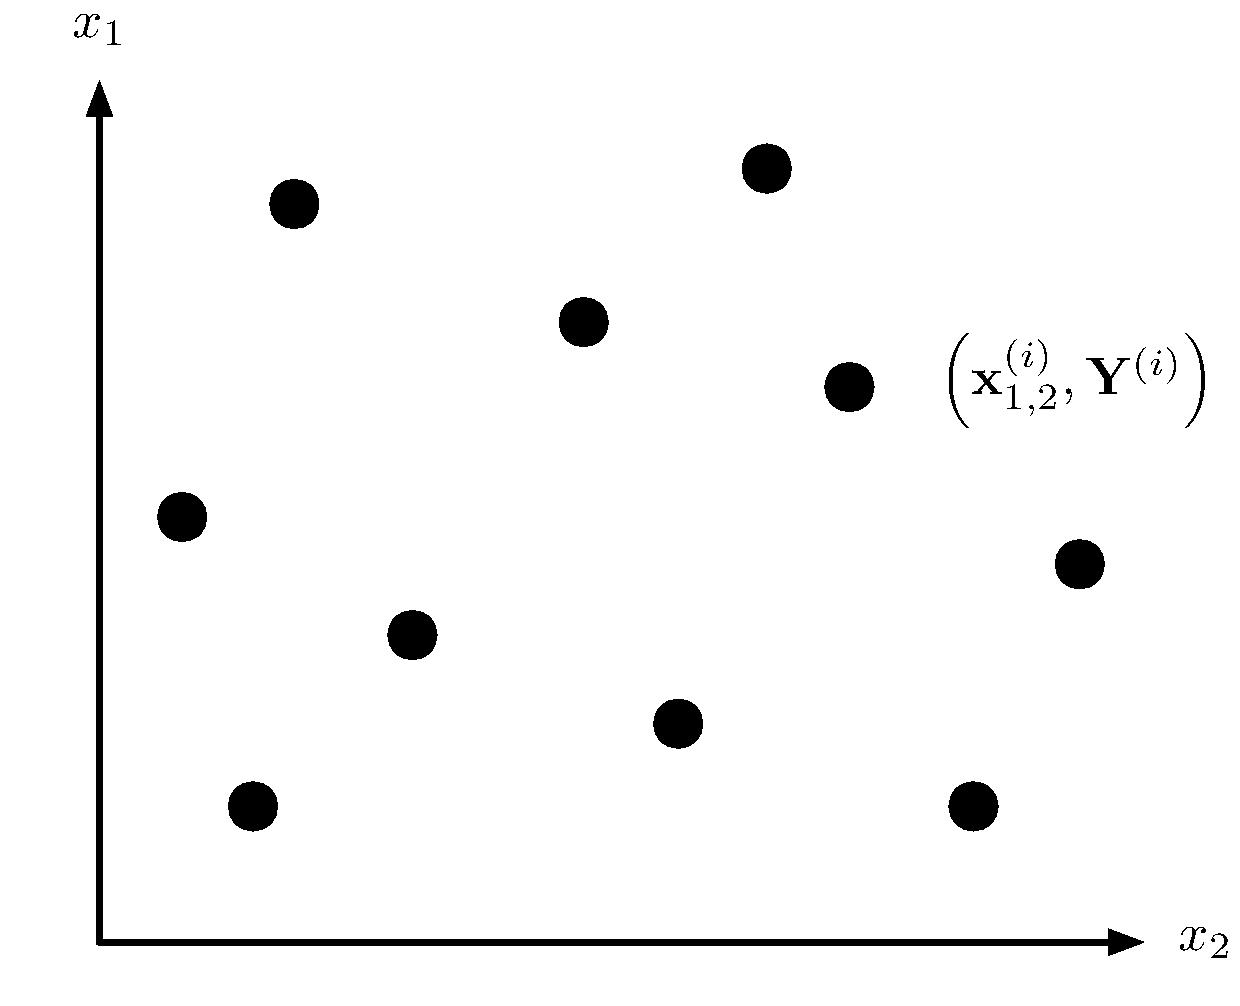
\includegraphics[width=0.5\linewidth,keepaspectratio]{fig/literature/doe.pdf}
\caption{Sketch of a 2-dimensional Design of Experiments.}
\label{fig:doe}
\end{figure}

In its basis form, a DoE is described by a $d$-dimensional cube: a hypercube---see~\cref{fig:hypercube}. A hypercube is parametrised by the minimal and maximal values of each parameters. In case parameters depends on each others, or if there are constrains on the parameters, non-rectangular domains~\citep{Lekivetz2015} have to be considered.

\begin{figure}[!h]
\centering
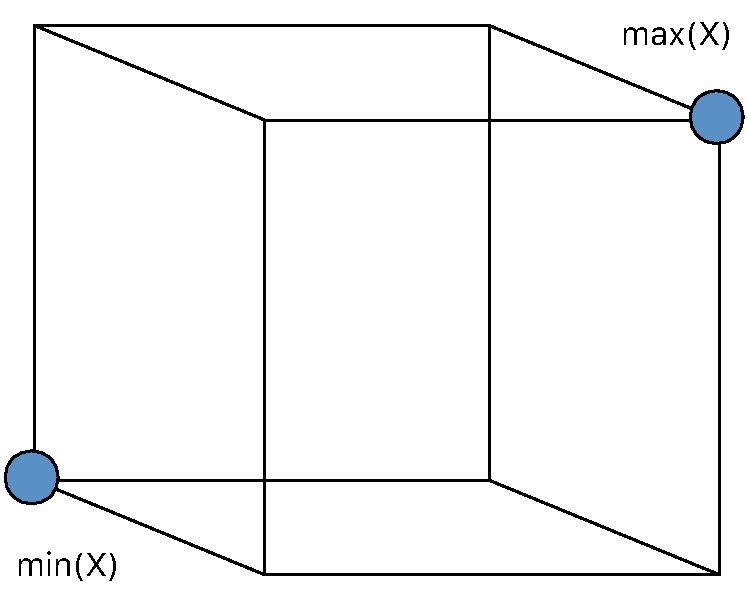
\includegraphics[width=0.5\linewidth,keepaspectratio]{fig/literature/hypercube.pdf}
\caption{Sketch of a 3-dimensional hypercube.}
\label{fig:hypercube}
\end{figure}

From exploratory phases to more advanced analyses, such as Uncertainty Quantification (UQ) and robust optimization, DoE aims at helping better understand the physical mechanisms governing the problem of interest~\citep{saltelli2007}. Therefore, the objective of efficient DoE is to maximize the coverage of the input space, i.e., space filling, with the aspiration of capturing most of the underlying physics. Such analyses typically require large number of experiments in order for the statistics of the QoIs to converge. In this regard, many studies have focused on trying to reduce the computational cost. However, depending on the required quality of the analysis, the complexity of the experiment, or its return time, the total number of experiments may be limited. Thus, the objective is to optimize the space-filling properties for a given number of experiments.

One-At-a-Time (OAT) design is the most trivial form of DoE. It consists in changing only one parameter at a time. While this method is simple to implement and allow a quick interpretation on a physical aspect, this sampling procedure require a huge number of simulation. Indeed, it requires $n^d$ samples. This exponential growth is called the \emph{cuse-of-dimensionality}. If we take for instance the unit-hypercube. All bounds range from 0 to 1. Let's say that we want to have a distance between each points of 0.01. The number of points required to fill the unit interval would be 100. In 2D the same spacing would require 10 000 and in 3D 1 000 000 points. As the number of dimensions goes, the number of experiments which is required to fill the space evenly rises exponentially as the volume of the space---see~\cref{fig:curse_dim}. To mitigate this problem, one could sparse the obtained DoE. The problem then comes to an assessment of the quality of this DoE.

\begin{figure}[!h]
\centering
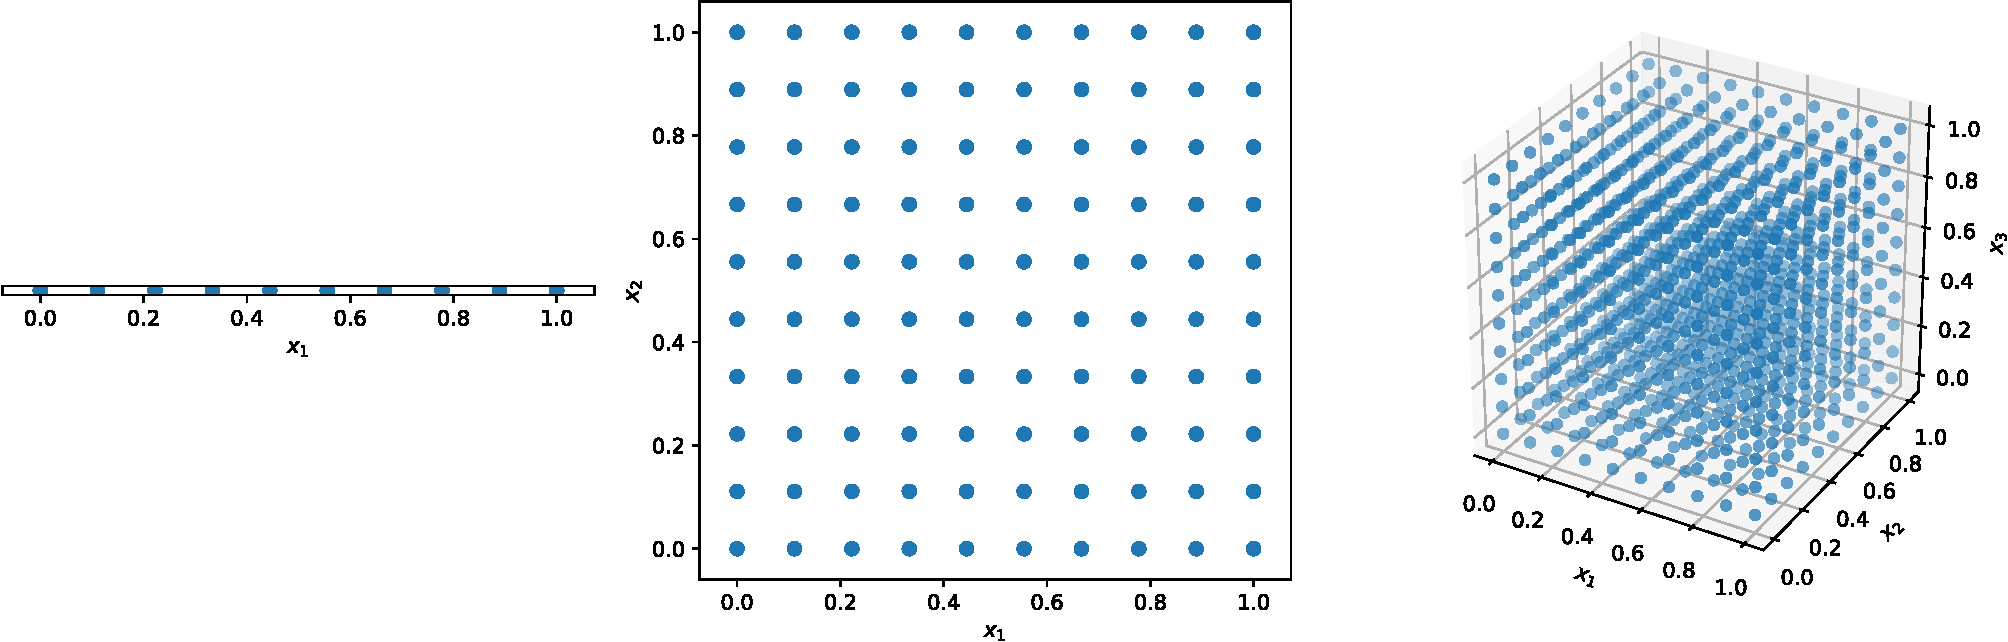
\includegraphics[width=0.8\linewidth,keepaspectratio]{fig/literature/curse_dim.pdf}
\caption{Sketch of the \emph{cuse-of-dimensionality}. VIsualization of the volume of the parameter space in 1, 2 and 3 dimensions.}
\label{fig:curse_dim}
\end{figure}

Different metrics are commonly used to assess the space filling of a DoE. They can be categorized into \emph{(i)} geometrical and \emph{(ii)} uniformity criteria. Among the most used geometrical criteria are the \emph{maximin} and \emph{minimax}~\citep{Pronzato2017}. They, respectively, maximize the minimal distance between all points or minimize the maximal distance between any location in space and all points of the sample. A similar criterion is found by using a \emph{minimum spanning tree}~\citep{Franco2009} in which the best design corresponds to a maximization of the mean distance between all connections and the minimization of the variance in these distances. The uniformity criterion, instead, measures how the spread of the points deviates from a uniform distribution. The central discrepancy is commonly used~\citep{Fang2006,Damblin2013} to measure the uniformity:
\begin{align}
C^2(\mathbf{X}^{N_s}_d) =& \left( \frac{13}{12} \right)^d - \frac{2}{N_s}\displaystyle\sum_{i=1}^{N_s}\prod_{k=1}^{d} \left( 1 + \frac{1}{2} \mid  x_k^{(i)} - 0.5\mid - \frac{1}{2} \mid  x_k^{(i)} - 0.5\mid^2\right)\\ \nonumber
& + \frac{1}{N_s^2}\sum_{i,j=1}^{N_s}\prod_{k=1}^d \left( 1 + \frac{1}{2} \mid  x_k^{(i)} - 0.5\mid + \frac{1}{2} \mid  x_k^{(j)} - 0.5\mid - \frac{1}{2} \mid  x_k^{(i)} - x_k^{(j)}\mid \right). \label{eq:c2}
\end{align}

There are three main methodologies for defining a DoE: \emph{(i)} \emph{Monte Carlo} (MC), \emph{(ii)} \emph{Latin Hypercube Sampling} (LHS) and \emph{(ii)} Quasi-\emph{Monte Carlo} (QMC) methods~\citep{Cavazzuti2013,Garud2017}. Kucherenko \emph{et al.}~\citep{Kucherenko2015} have recently compared MC and LHS against the well-established low discrepancy sequence of \emph{Sobol'}. They concluded that LHS and QMC both offer superior integration performance over MC.

LHS-based sampling methods are one-shot design strategies~\citep{Mckay1979,Fang2006}. The principle is simple: considering $N_s$ samples, in each 1-dimensional subprojection of the parameter space there should be $N_s$ samples. It means that samples are not sharing coordinates with each other. Orthogonal arrays are a slight evolution of this principle. Each 1-dimensional subprojection is spitted into $N_s$ to form an orthogonal grid of size $N_s^d$ and only one sample is allowed per cell. \Cref{fig:lhs} shows two different orthogonal LHS with $N_s=10$. Although both valid, they do not cover equally the parameter space. Constructing such design is numerically easy and it is possible to optimize the space filling properties by swapping elements for instance~\cite{Fang2006,Damblin2013}.

\begin{figure}[!h]               
\centering
\subfloat[]{
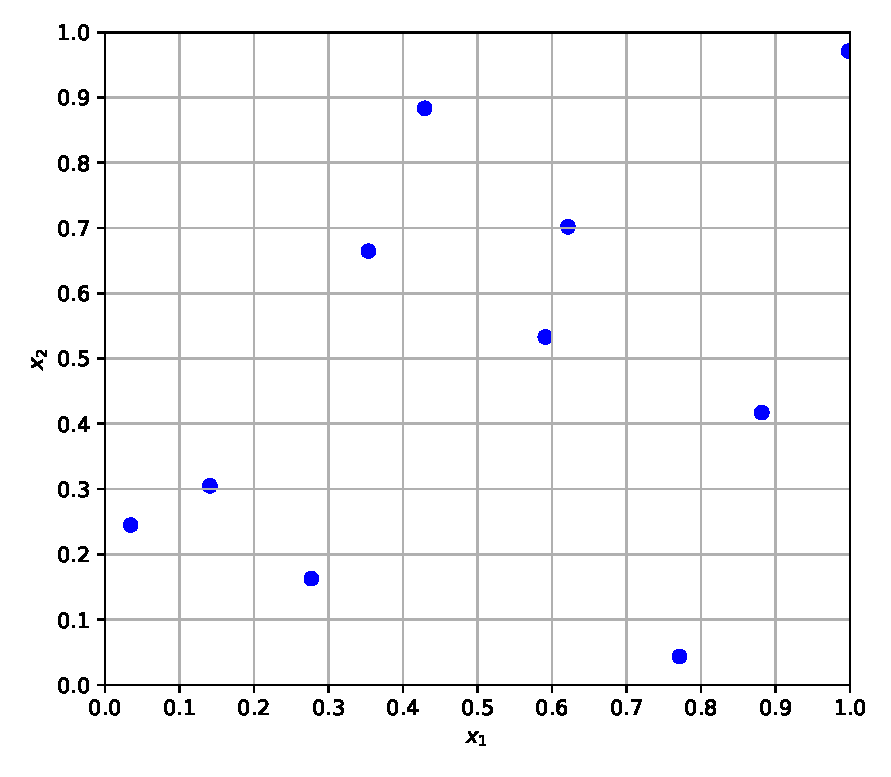
\includegraphics[width=0.47\linewidth,height=\textheight,keepaspectratio]{fig/literature/lhs_ok.pdf}}
 ~       
\subfloat[]{
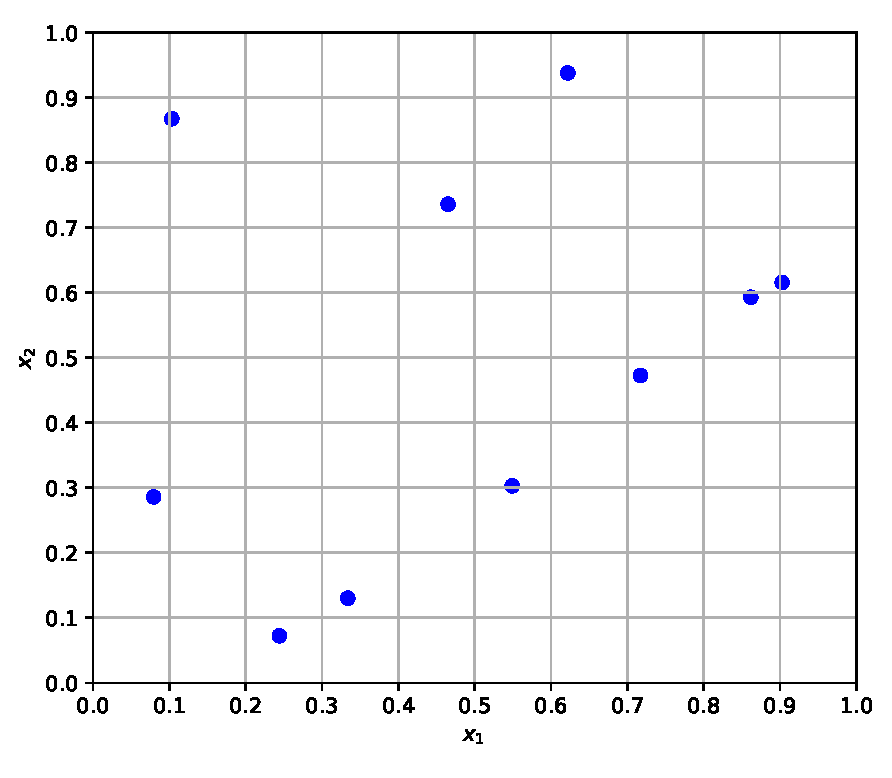
\includegraphics[width=0.47\linewidth,height=\textheight,keepaspectratio]{fig/literature/lhs_ko.pdf}}
\caption{Orthogonal LHS examples.}
\label{fig:lhs}
\end{figure}

The use of LHS requires the practitioner to set \emph{a priori} the total number of samples contained in the DoE. Although, there have been some attempts to construct progressive LHS, they still require an initial design to work properly~\citep{Sheikholeslami2017}.

On the other hand, low discrepancy sequences are iterative designs which can be continued without compromising the discrepancy. The practitioner is then able to increase the number of samples afterwards for quality reasons, for instance, or if other experiments can be afforded. \citet{Liu2018} recently reviewed iterative DoE in a metamodeling context. In their study, it is shown that most iterative methods need an initial design as a starting point. A particular benefit of this approach is that it allows the use of physics information from the system to guide further exploration of the DoE. In this case, such iterative methods are called adaptive methods. Except for some work in~\citep{Crombecq2011}, and to the best of the authors’ knowledge, the number of iterative methods not requiring an initial design is limited. This state-of-the-art can be explained both by the quality of the initial designs (using LHS of \emph{Sobol'} sequence) and by the performance of the refinement algorithm. There are even fewer options if the iterative design cannot take advantage of the output of the experiments. Low discrepancy sequences are an example of such methods. But in some context, stochastic methods may be required ---\thinspace to compute sensitivity indices for instance~\citep{Saltelli2010}. Scrambling the sequences~\citep{Owen1998} can avoid this pitfall but then the method is no longer iterative.

\section{Uncertainty Quantification}\label{sec:uq}

\subsection{Uncertainty Propagation}\label{sec:up}
\lettrine{U}{ncertainty Propagation} (UP) seeks to communicate uncertainties throughout the system. Uncertainties are defined at one side of the system, and their effects are observed at the other end. But are we talking about the uncertainties of the input parameters or the output QoI? Usually, uncertainties are defined on the input parameter space side, and it is the impact on the quantity of interest that is observed. The other way around is called an \emph{inverse problem} and is not discussed in this work.

Uncertainties can be described using a probabilistic approach through the use of Probability Density Functions (PDF). This function computes the probability of occurence of a phenomenon. Thus, propagating uncertainties comes to determining the PDF of the QoI.

\begin{figure}[!h]
\centering
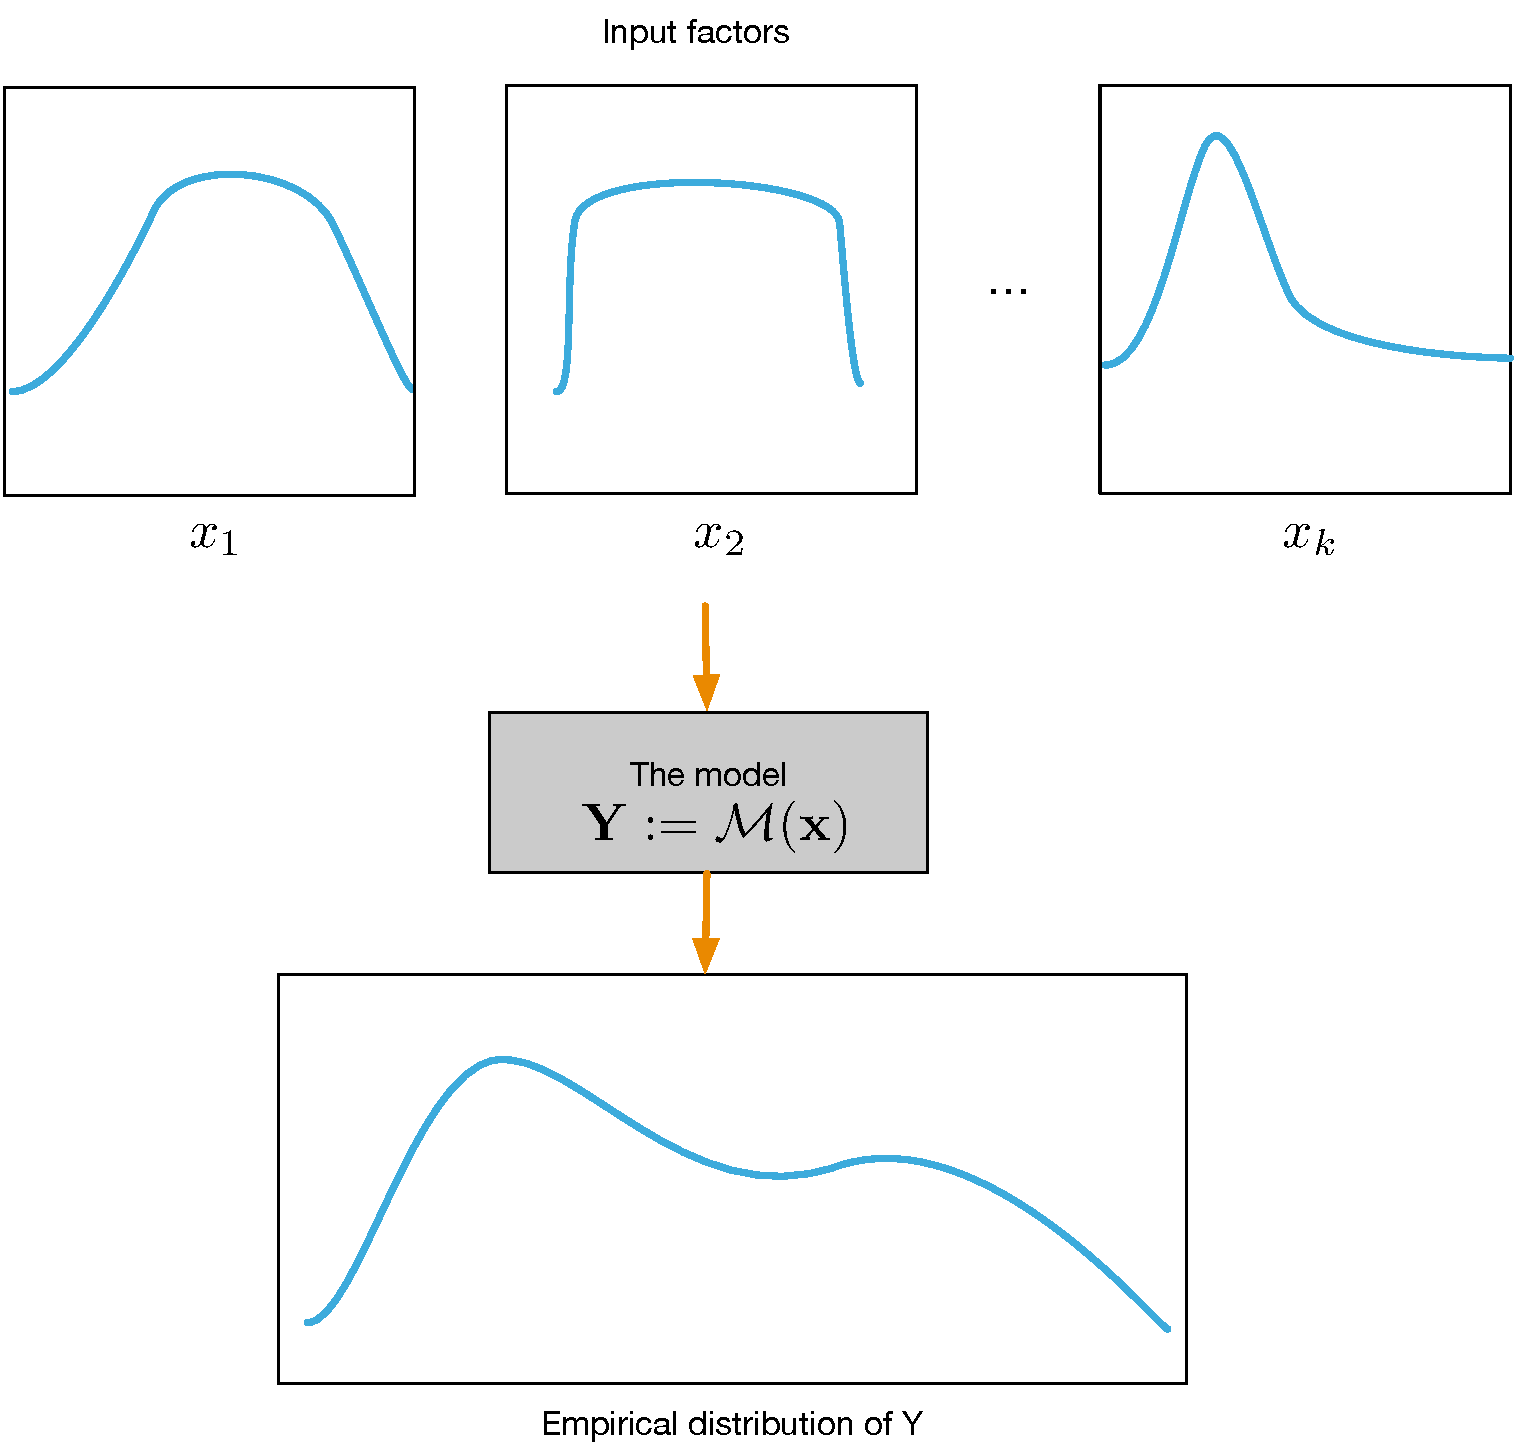
\includegraphics[width=0.7\linewidth,keepaspectratio]{fig/literature/propagation.pdf}
\caption{Sketch of the Uncertainty Propagation procedure.}
\label{fig:UP}
\end{figure}

\Cref{fig:UP} present a representation of the UP procedure. In practice, propagating uncertainties comes to sampling the PDFs of inputs and observing the impact on the QoI. It should be emphasised that the outcome of the UP \emph{depends} on the prescribed PDFs. The nature of the PDF and the ranges of each parameters is paramount. Without any prior knowledge on input parameters, uniform distributions are traditionally used. As for the ranges, some fixed percentage of variation is commonly used. While this strategy could indeed corresponds to the correct variability of some parameters, this may lead to wrong analysis. In~\citep{pilkey}, the exemple of radioactive waste transport on the Yucca Mountain is taken. In this UP analysis, the percolation rate of the water from the surface to the disposal was wrongly estimated between 0.02 and 1 millimetre per year while its true was close to $\sim 3000$. This lead to an underestimation of 4 orders of magnitude of the transport of some radioactive component.

As we are interested in computing statistics on the QoI, this requires a statistically significant sampling. A high number of samples is required to recover the empirical PDF of the QoI. One must note that in order to find the tail of the PDF---the least frequent event---it requires an even larger number of samples.

Histograms can be used to represent the PDF. However, continuous functions can be obtained using a technique called Kernel Density Estimation (KDE)~\cite{Wand1995}. The probability to observe a QoI's value $Y^*$ is given by the PDF estimator $\hat{f}(Y^*)$
\begin{align}
\hat{f}(Y^*)&= \frac{1}{N_{s}}\sum_{i=1}^{N_{s}} K_{h_i}(Y^*-Y^{(i)}),
\end{align}
\noindent where $N_s$ is the number of samples. $K_{h_i}(.) = K(./h_i)/h_i$ is the scaled kernel chosen for the modal probability density function with $h_{i}$ the bandwidth for the \emph{i}th component. In the present work $K$ is the Gaussian kernel and $h_{i}$ are optimized by cross-validation of the log-likelihood of the data. It writes
\begin{align}
K\left(Y^*,Y^{(i)}\right) = \exp\left( - \frac{D\left(Y^*,Y^{(i)}\right)^2}{2h^2} \right), \label{eq:kde}
\end{align}
\noindent with $D$ a distance function. It should be noted that estimating the density in a high dimensional parameter space is challenging~\citep{Scholkopf1999,Scott2015}. See \cref{sec:visu} for a $n$-dimensional representation of the PDF.

Depending on the number of sample available and on the parameters of the method, this process can lead to a PDF which is far from the real one. The principle is fairly easy to understand---see~\cref{fig:kde}. Each sample value $Y$ is represented on the $x$-axis. Around each value, a rectangle of fixed width and fixed height is draw. When there is an overlap, the rectangle values are summed-up. The value of the width represents the bandwidth, and the general shape of the \emph{rectangle} is called the kernel. As previously stated, Gaussian kernel is classically used and corresponds to a bell-cuve shape.

\begin{figure}[!h]
\centering
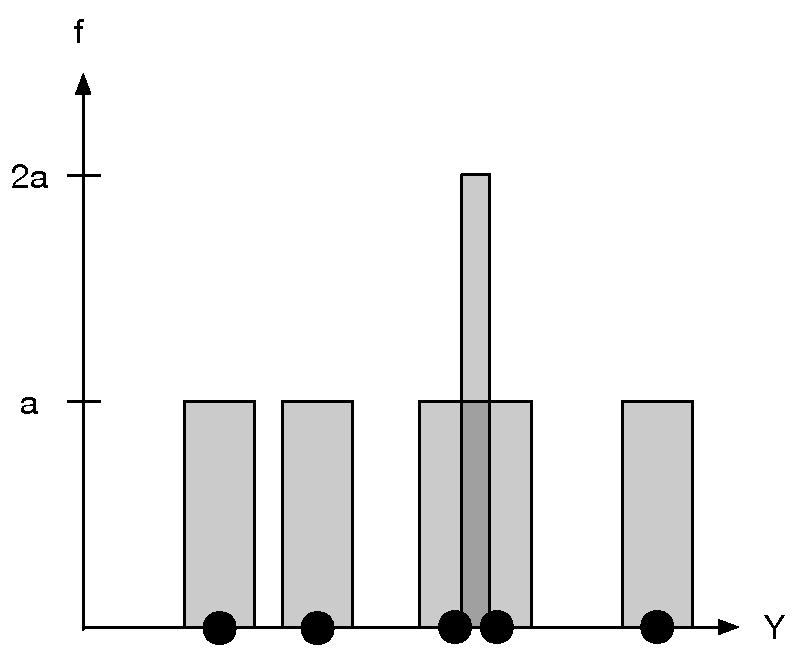
\includegraphics[width=0.6\linewidth,keepaspectratio]{fig/literature/kde.pdf}
\caption{Sketch of a Kernel Density Estimation procedure with a rectangular kernel.}
\label{fig:kde}
\end{figure}

\Cref{fig:ex_pdf}(a) presents a KDE of a 1-dimensional QoI along with a histogram representation of the data. It can be seen that the KDE act as a smoothing procedure of the histogram. Another possibility---\cref{fig:ex_pdf}(b)---is to use quantile dotplot \cite{kay2016} which allows to directly count the quantiles. In this example, there are 20 circles, and below $F=22.5$ there are 11 circles. Thus, >50\% of the samples are located below $F=22.5$.

\begin{figure}[!h]               
\centering
\subfloat[Kernel Density Estimation and histogram]{
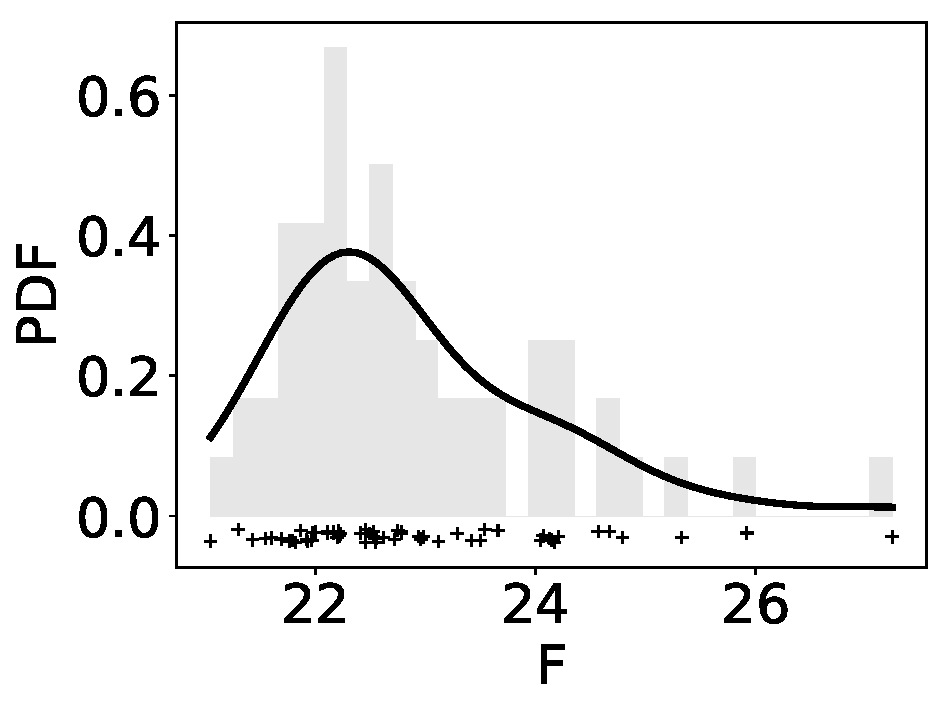
\includegraphics[width=0.47\linewidth,height=\textheight,keepaspectratio]{fig/literature/pdf_hist.pdf}}
 ~       
\subfloat[Kernel Density Estimation and quantile dotplot]{
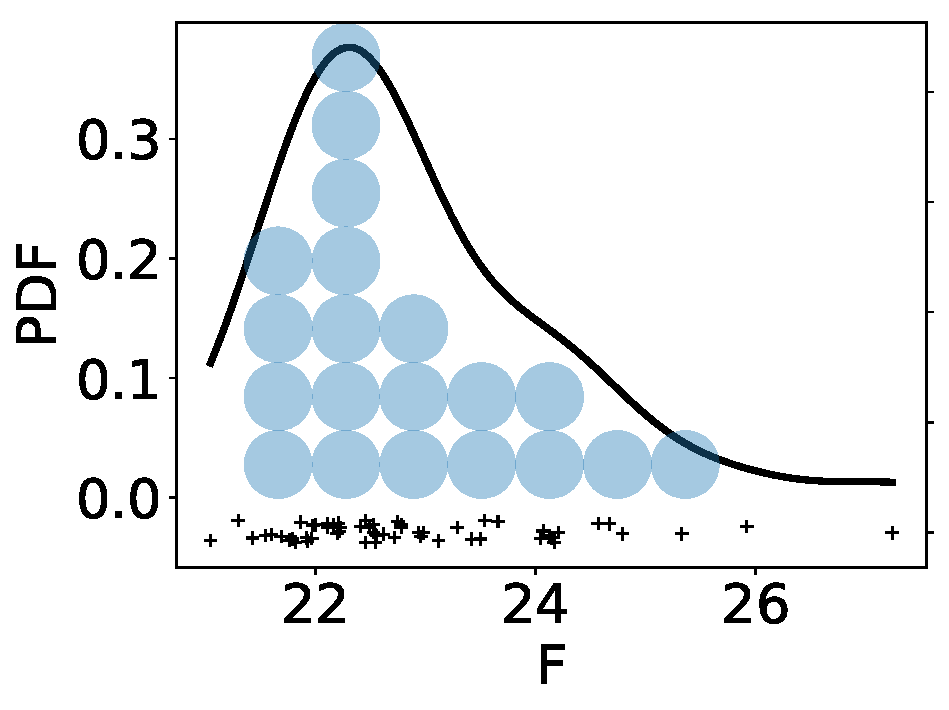
\includegraphics[width=0.47\linewidth,height=\textheight,keepaspectratio]{fig/literature/pdf_dotplot.pdf}}
\caption{Visualization of a 1-dimensional PDF.}
\label{fig:ex_pdf}
\end{figure}

Once the PDF of the QoI is available, it can be used to: \emph{(i)} observe the probability to exceed a threashold; \emph{(ii)} compute the probability to have a certain event; or just \emph{(iii)} get general statistics (mean, variance, quantiles).

\subsection{Sensitivity Analysis}\label{sec:sa}
\lettrine{S}{ensitivity Analysis} (SA) refers to the determination of the contribution of different parameters on quantities of interest~\cite{saltelli2007,iooss2016}. The most natural way to do SA would be to consider the derivatives. But this information is known to be to local or general---although there are some work extending the capabilities of these methods~\cite{kucherenko2016}. In the literature, a distinction is made between local and global SA. In the following both local-based SA (derivative) and global-based SA (variance-based and moments-based) methods are presented.

\subsubsection{From local to global Sensitivity Analysis}

An intuitive way to characterize the importance of each parameters toward a QoI is to compute the derivates of the simulator for a given set of inputs. This method is called \emph{elementary effects} and a successful implementation is found with \citet{morris1991}. An elementary effect $d\mathbf{x}_{k}^*$ is defined as
\begin{align}
d\mathbf{x}_{k}^* = \frac{ \mid Y(\mathbf{x}_{k}^*) -  Y(\mathbf{x}_{k}) \mid}{\mid \mathbf{x}_{k}^* - \mathbf{x}_{k}  \mid},
\end{align}
\noindent with $\mathbf{x}_{k}$ a given sample and $\mathbf{x}_{k}^*$ a sample which differs from $\mathbf{x}_{k}$ by an increment $\delta$. This effect can be computed with respect to $N_s$ samples and $d$ dimensions which induce to a total number of sample $N = N_s\times(d + 1)$. It is called a screening method and it corresponds to an OAT walk of the DoE. \Cref{fig:morris} is an example with $N_s = 5, d = 3$. Then the mean of absolute elementary effects writes
\begin{align}
\hat{\mu_k} = \frac{1}{N_s} \sum_{i=1}^{N_s} \frac{ \mid Y(\mathbf{x}_{k}^*) -  Y(\mathbf{x}_{k}^i) \mid}{\mid \mathbf{x}_{k}^* - \mathbf{x}_{k}^i  \mid}.
\end{align}

\begin{figure}[!h]
\centering
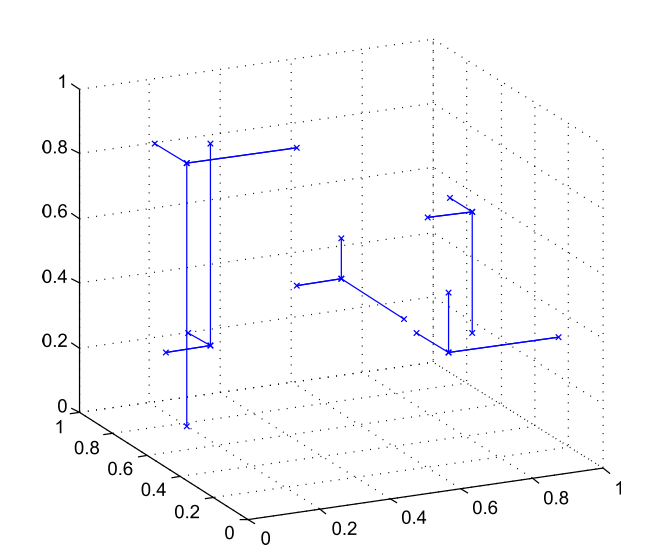
\includegraphics[width=0.8\linewidth,keepaspectratio]{fig/literature/morris.png}
\caption{Sketch of \emph{Morris}' screening method. Source~\cite{Becker2018}.}
\label{fig:morris}
\end{figure}

A popular extension of this method is found with the derivative-based global sensitivity measures (DGSM)~\cite{kucherenko2016,Becker2018}. Although these methods perform well in high dimensions and with a low sampling size, they are not exempt of flaws. As local methods, the construction of the indices is based on local OAT variations which are not able to take into account correctly correlations between the input parameters.

\subsubsection{Variance-based Sensitivity Analysis}
Variance-based Sensitivity Analysis allows to obtain the contribution of the parameters on the QoI's variance~\cite{ferretti2016}. Here, classical \textit{Sobol'}~\cite{Sobol1993} method is presented which gives not only a ranking but also quantifies the importance factor using the variance. This method makes the hypothesis of the independence of the input variables. It uses a functional decomposition of the variance of the function to explore
\begin{align}
\mathbb{V}(Y) &= \sum_{i}^{d} \mathbb{V}_i (Y) + \sum_{i<j}^{d}\mathbb{V}_{ij}(Y) + ... + \mathbb{V}_{1,2,...,d}(Y),
\end{align}
\noindent introducing conditional variances:
\begin{align}
\mathbb{V}_i(Y) &= \mathbb{\mathbb{V}}[\mathbb{E}(Y|x_i)]\nonumber\\
\mathbb{V}_{ij}(Y) &= \mathbb{\mathbb{V}}[\mathbb{E}(Y|x_i x_j)] - \mathbb{V}_i(Y) - \mathbb{V}_j(Y),\nonumber
\end{align}
\noindent \textit{Sobol'} indices are expressed as
\begin{align}
S_i = \frac{\mathbb{V}_i(Y)}{\mathbb{V}[Y]}\qquad S_{ij} = \frac{\mathbb{V}_{ij}(Y)}{\mathbb{V}[Y]}.
\end{align}
\noindent $S_{i}$ corresponds to the first order term which apprises the contribution of the \textit{i-th} parameter, while $S_{ij}$ corresponds to the second order term which informs about the correlations between the \textit{i-th} and the \textit{j-th} parameters. These equations can be generalized to compute higher order terms. However, the computational effort to converge them is most often not at hand and their analysis and interpretations are not simple.

Total indices represents the global contribution of the parameters on the variance of the QoI and express as:
\begin{align}
S_{T_i} = S_i + \sum_j S_{ij} + \sum_{j,k} S_{ijk} + ... = 1 - \frac{\mathbb{V}[\mathbb{E}(Y|x_{\sim i})]}{\mathbb{V}[Y]}.
\end{align}

\Cref{fig:sobol}(a) is an example using \textit{Ishigami} function~\cite{ishigami1990}
\begin{align}
Y(\mathbf{x}) = \sin x_1 + 7 \sin^2 x_2 + 0.1 x_3^4 \sin x_1,
\end{align}
\noindent with $\mathbf{x} \in [-\pi, \pi]^3$. This function exhibits strong nonlinearity and nonmonotonicity. It is particularly interesting because the first order indice of $S_{x_3} = 0$ whereas it's total order is $S_{T_{x_3}} = 0.244$. Note that on second order indices, $S_{x_1,x_3} = 0.244$. It means that almost 25\% of the observed variance on the QoI is due to the correlations between $x_3$ and $x_1$, although $x_3$ by itself has no impact on the QoI.

Looking at \cref{fig:sobol}(b), it can be noted that the convergence of these indices require a large sampling size. The required sampling size is case dependant as it depends on the number of input parameters and on the complexity of the function of interest.

\Cref{fig:scatter_sobol} gives a visual explanation of \emph{Sobol'} indices. It shows scatter plots of the output with respect to each parameter. By conditioning the output value by given values of the parameter (\emph{black lines}), the conditional output mean is computed. It corresponds to the term $\mathbb{E}(Y|x_i)]$. Taking the variance of this term gives the numerator of the \emph{Sobol'} indices. Looking at $x_3$, the variance of the mean is close to zero leading to $S_{x_3} = 0$. But we can further observe that the variance of the output is not constant along the parameter values of $x_3$. This heteroscedasticity is explained by higher order interactions. Moreover, an heteroscedasticity is also noticeable on $x_1$ leading to an interaction between $x_3$ and $x_1$. On $x_2$, the variance seems to be constant and thus null interaction with this parameter can be supposed. This case is fairly simple to analyse visually---although it is only a qualitative analysis. Nevertheless, when the number of input parameters increases such analysis becomes unrealistic as it would be difficult to conclude on high order terms.

\begin{figure}[!h]               
\centering
\subfloat[First and total \textit{Sobol'} indices]{
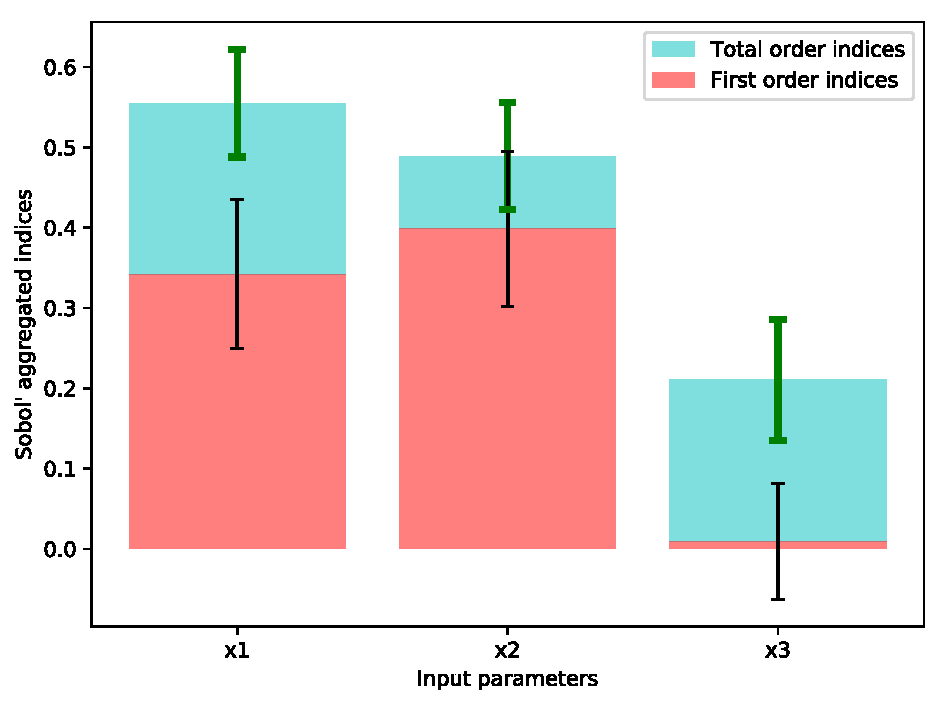
\includegraphics[width=0.47\linewidth,height=\textheight,keepaspectratio]{fig/literature/sobol_aggregated.pdf}}
~
\subfloat[Convergence of the \emph{Sobol'} indices]{
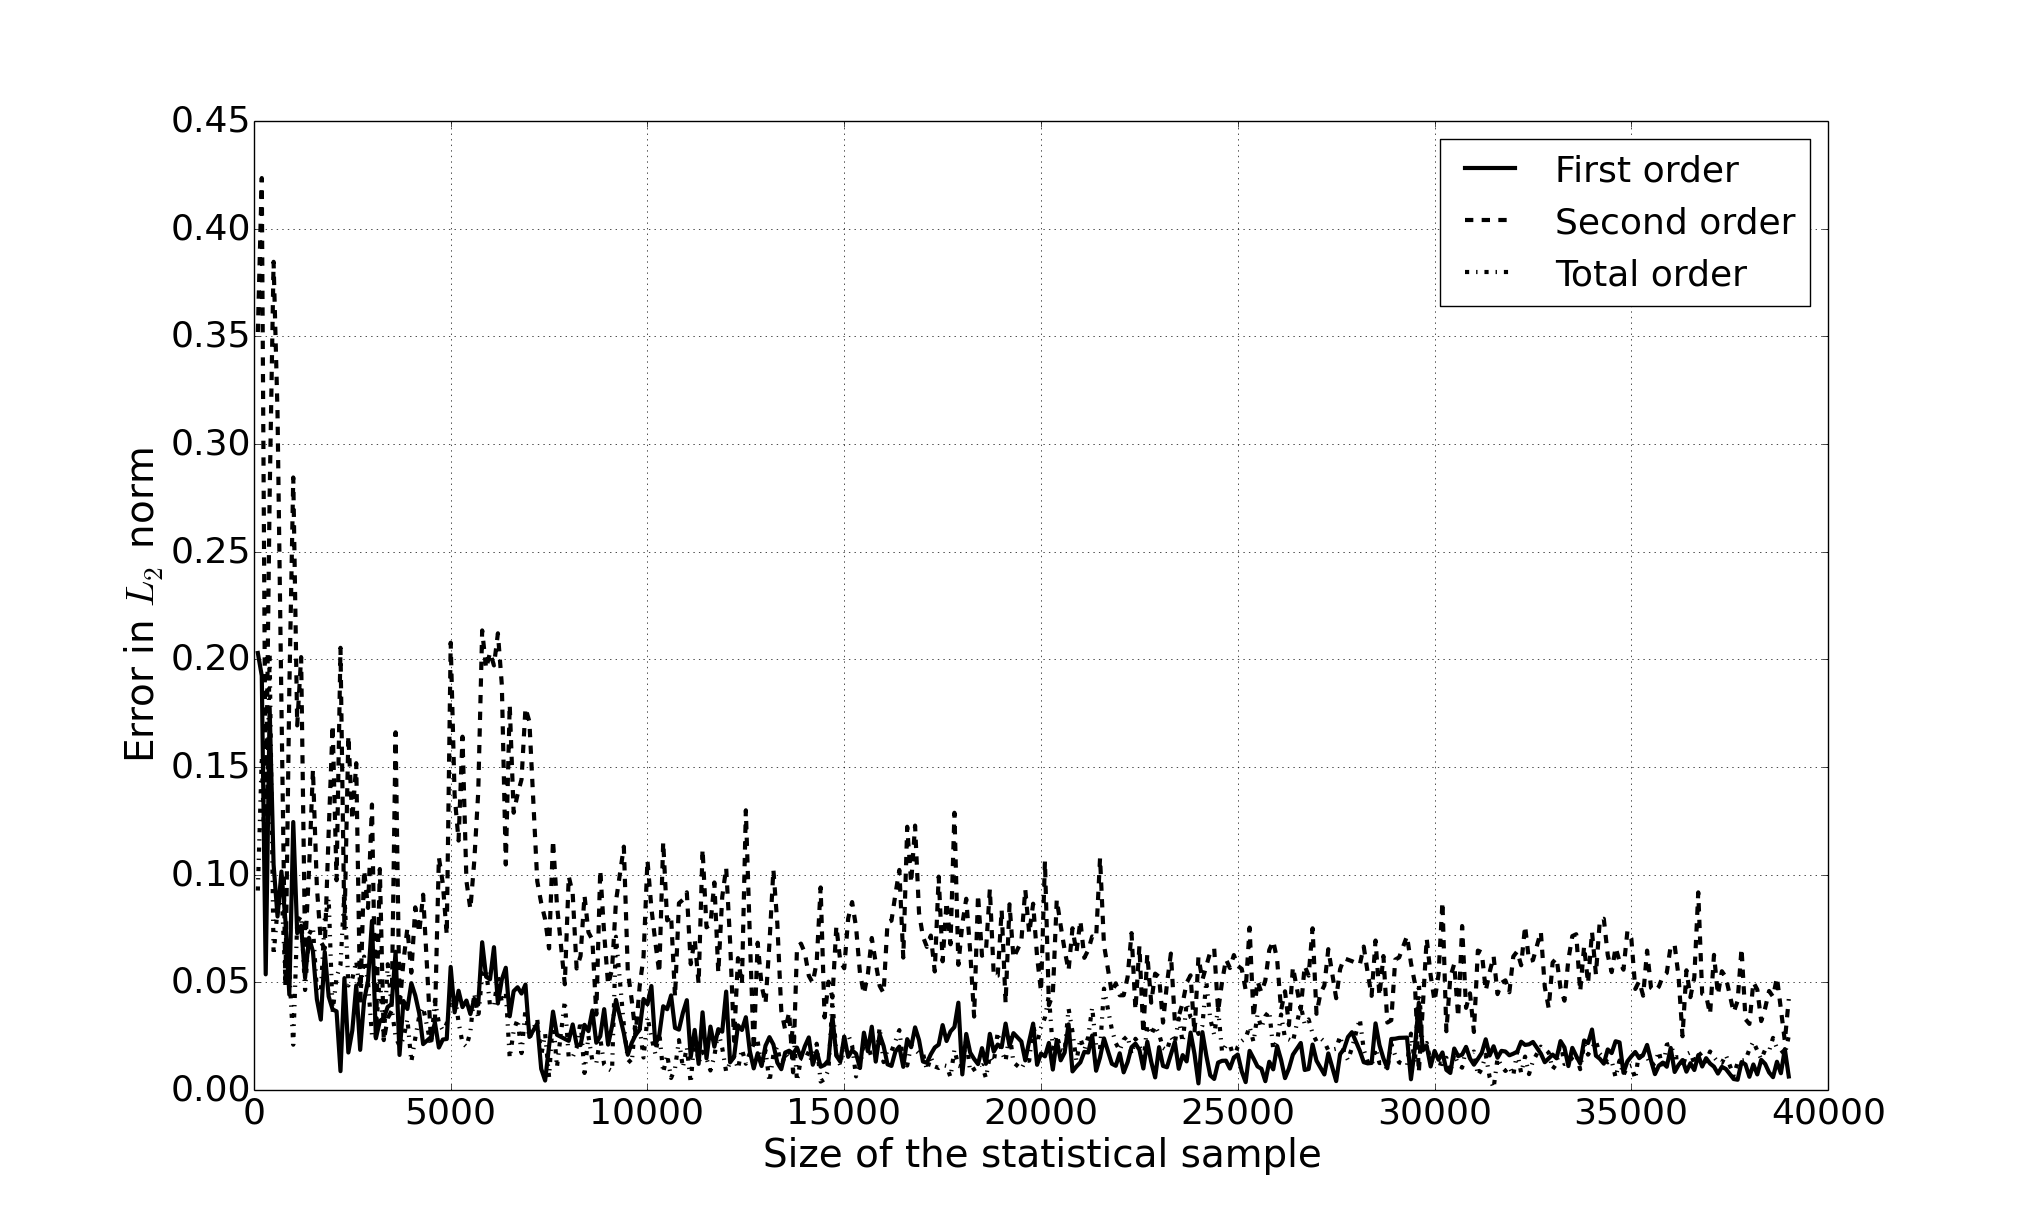
\includegraphics[width=0.47\linewidth,height=\textheight,keepaspectratio]{fig/literature/l2_sample.png}}
\caption{First and total \textit{Sobol'} indices on the Ishigami function.}
\label{fig:sobol}
\end{figure}


\begin{figure}[!h]
\centering
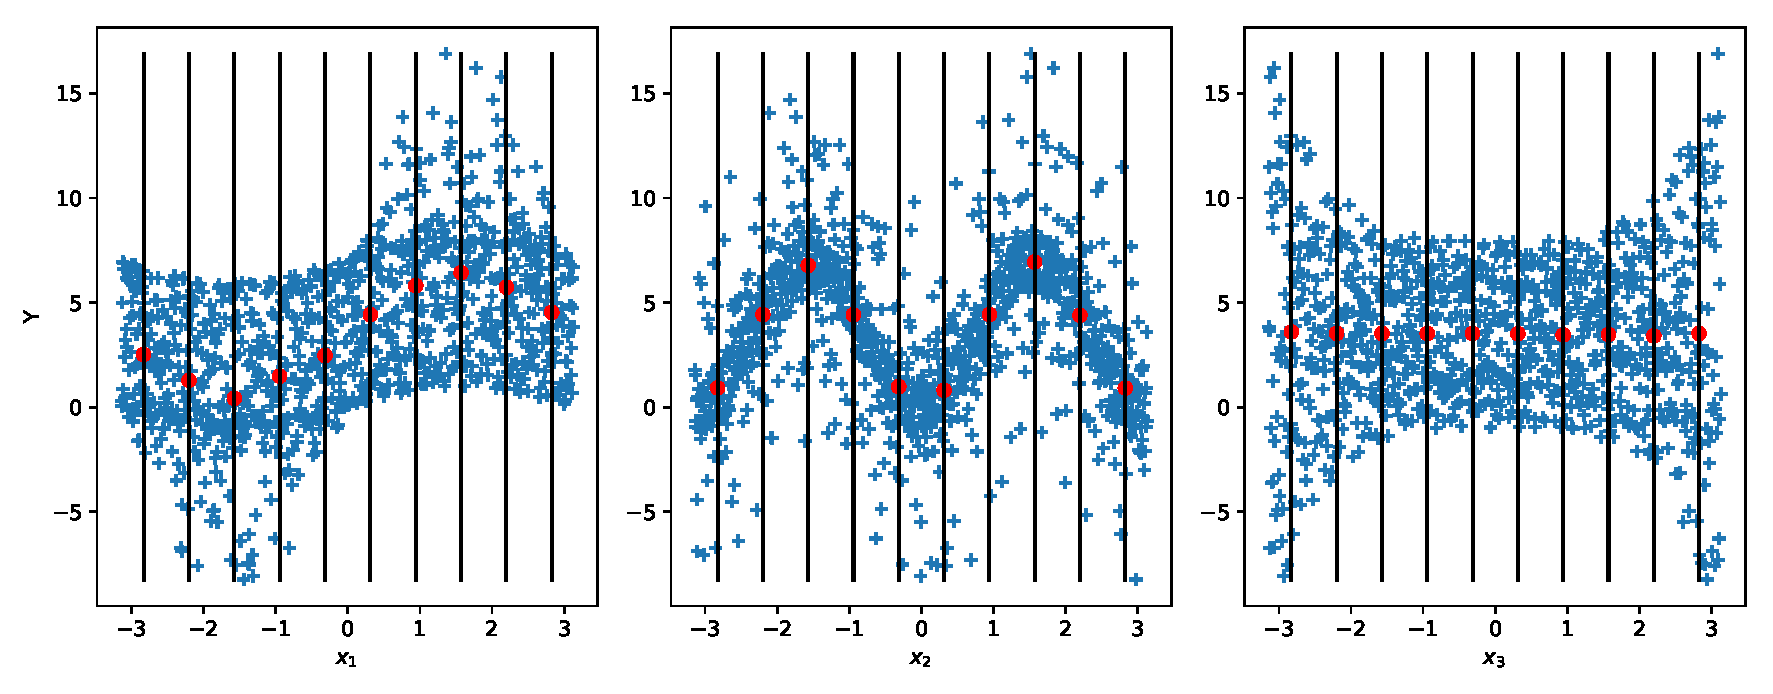
\includegraphics[width=\linewidth,keepaspectratio]{fig/literature/scatter_sobol.pdf}
\caption{Scatter plot per component of the \textit{Ishigami} function. \emph{Blue crosses} represent the outputs, \emph{black lines} the conditioning over a given parameter, \emph{red dots} the mean given a conditioning.}
\label{fig:scatter_sobol}
\end{figure}

Classical empirical formulations of \emph{Sobol'} indices require the use of 3 (resp. 4) matrices to compute first and total (resp. and second order indices)~\cite{Saltelli2010}. The computation requires two independent sampling $A$, $B$ of size $N$ and a matrice $AB$ which is a combination of both matrices (resp. $BA$). $AB_{n}$ corresponds to the matrice $A$ with the column $n$ from the matrice $B$. Hence the number of forward model evaluation is $N_s = N(d + 2)$. In~\citep{baudin2016}, they showed that \textit{Martinez}' formulation is stable and provides asymptotic confidence intervals---approximated with Fisher's transformation---for first order and total order indices. \textit{Martinez}' estimators write
\begin{align}
\hat{S_i} = \rho (Y(B), Y(AB_{n})) \quad \hat{S_{T_i}} = 1 - \rho (Y(A), Y(AB_n)),
\end{align}
\noindent where $\rho$ is the linear correlation coefficient.

For a functional output, as for the \textit{LS89} blade case---see~\cref{chap:ls89} and \cref{fig:map_sobol}---, \textit{Sobol'} indices can be computed all along the output vector and retrieve a map or create composite indices. As described by Marrel~\cite{marrel2015}, aggregated indices can also be computed as the mean of the indices weighted by the variance at each point or temporal step
\begin{align}
S_i = \frac{\displaystyle\sum_{l = 1}^{m} \mathbb{V} [\mathbf{Y}^l] S_i^{l}}{\displaystyle\sum_{l = 1}^{m} \mathbb{V} [\mathbf{Y}^l]}.
\end{align}

\begin{figure}[H]
\centering
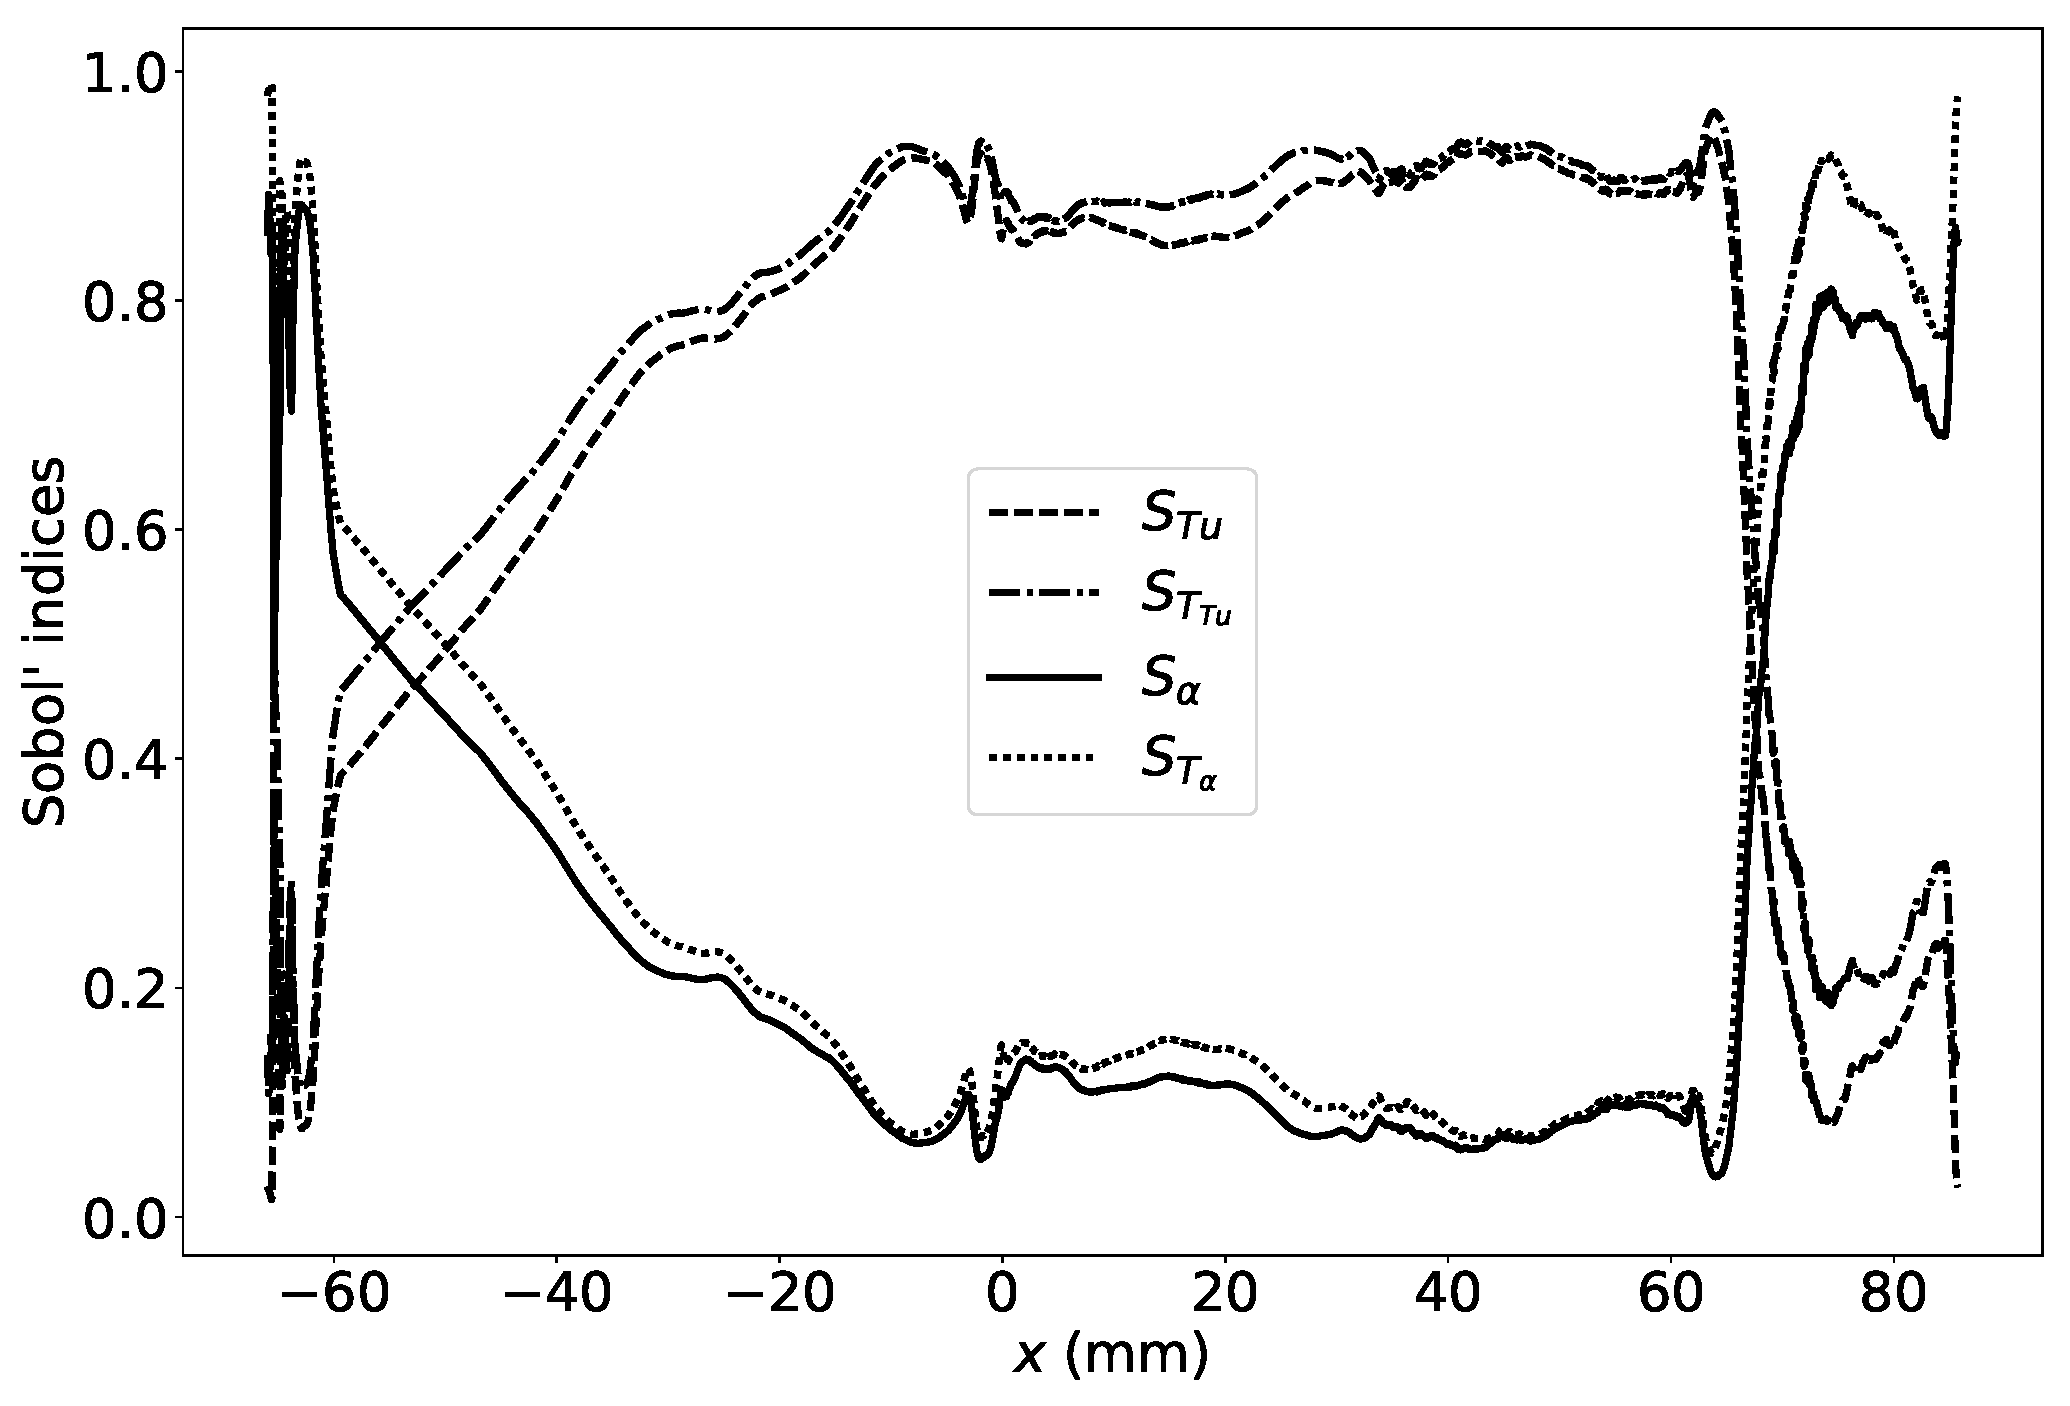
\includegraphics[width=0.8\linewidth,keepaspectratio]{fig/literature/sobol_map.pdf}
\caption{Map of \emph{Sobol'} indices along the \textit{LS89} blade.}
\label{fig:map_sobol}
\end{figure}

\subsubsection{Moment-based Sensitivity Analysis}
Variance-based SA are standard methods (although elementary effects or classical regression are still commonly used among practitioners~\cite{ferretti2016}) but they do not come without flaws~\cite{borgonovo2016}:

\begin{itemize}
\item \emph{Only the second order moment is taken into account,}\\
It means that if the QoI's PDF is highly skewed, multimodal or with heteroscedastic data, this information will be lost. Hence, the variance is only a good measure if the distribution is close to normal.
\item \emph{The parameters need to be uncorrelated,}\\
This assumption can be mitigated by using some correlation matrices but the procedure is not really trivial.
\item \emph{Null first order indices does not imply that the parameter is independent with the QoI,}\\
Computation of high order terms and total effect require a lot of samples to converge. It may be impractical to compute these quantities.
\end{itemize}

Moment-based method are based on the whole PDF to mitigate these issues~\cite{borgonovo2007}. Based on the unconditional PDF, a conditional PDF per parameter is computed. The more the conditional PDF deviates from the unconditional PDF, the more the parameter has an impact on the quantity of interest. The same procedure can be done using the Empirical Cumulative Density Function (ECDF), respectively with the unconditional ECDF. \Cref{fig:scatter_moments} visually shows this procedure. Bins of samples (\emph{red circles}) are used to compute a conditional PDF of the output. This PDF is compared to the unconditional PDF.

\begin{figure}[!h]
\centering
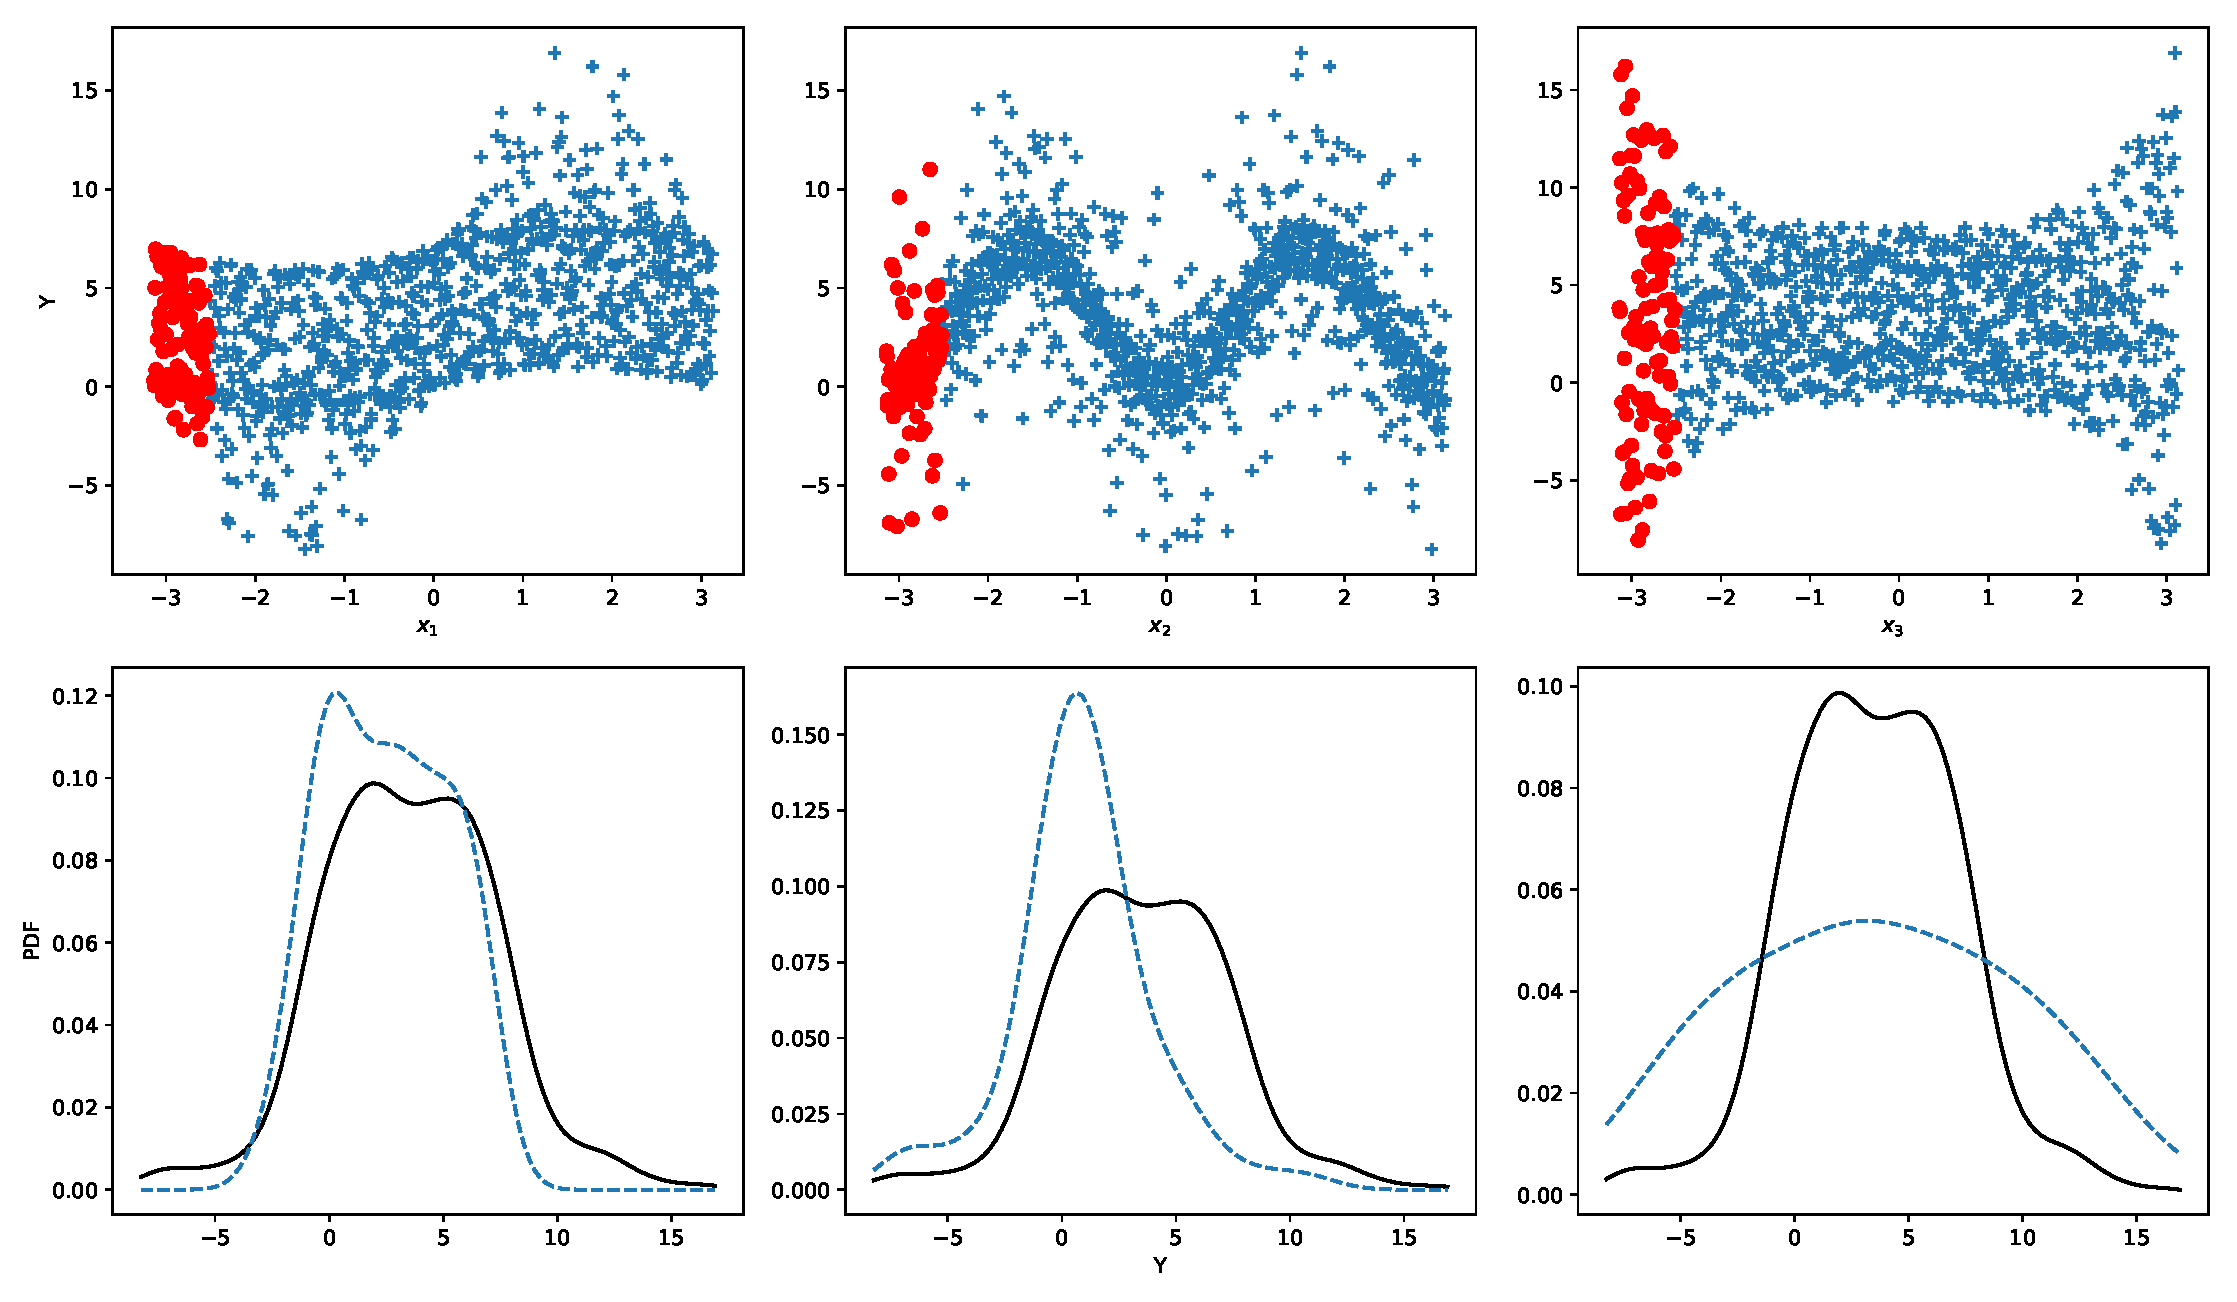
\includegraphics[width=\linewidth,keepaspectratio]{fig/literature/scatter_moments.pdf}
\caption{Scatter plot per component of the \textit{Ishigami} function. \emph{Black line} represents the unconditional PDF and \emph{red dots} the samples used to computed the conditioned PDF (\emph{dashed line}).}
\label{fig:scatter_moments}
\end{figure}

\Cref{fig:moment_sa} shows the computation of both conditional and unconditional PDF (resp. ECDF). Based on these moment estimations, distance criteria can be computed such as: $L_1$, \emph{Kolmogorov-Smirnov} or the \emph{Kuiper} distances. The method does not require any particular sampling nor do not require the parameters to be independent. The limitations comes from the ability to correctly estimate the densities.

\begin{figure}[!h]
\centering
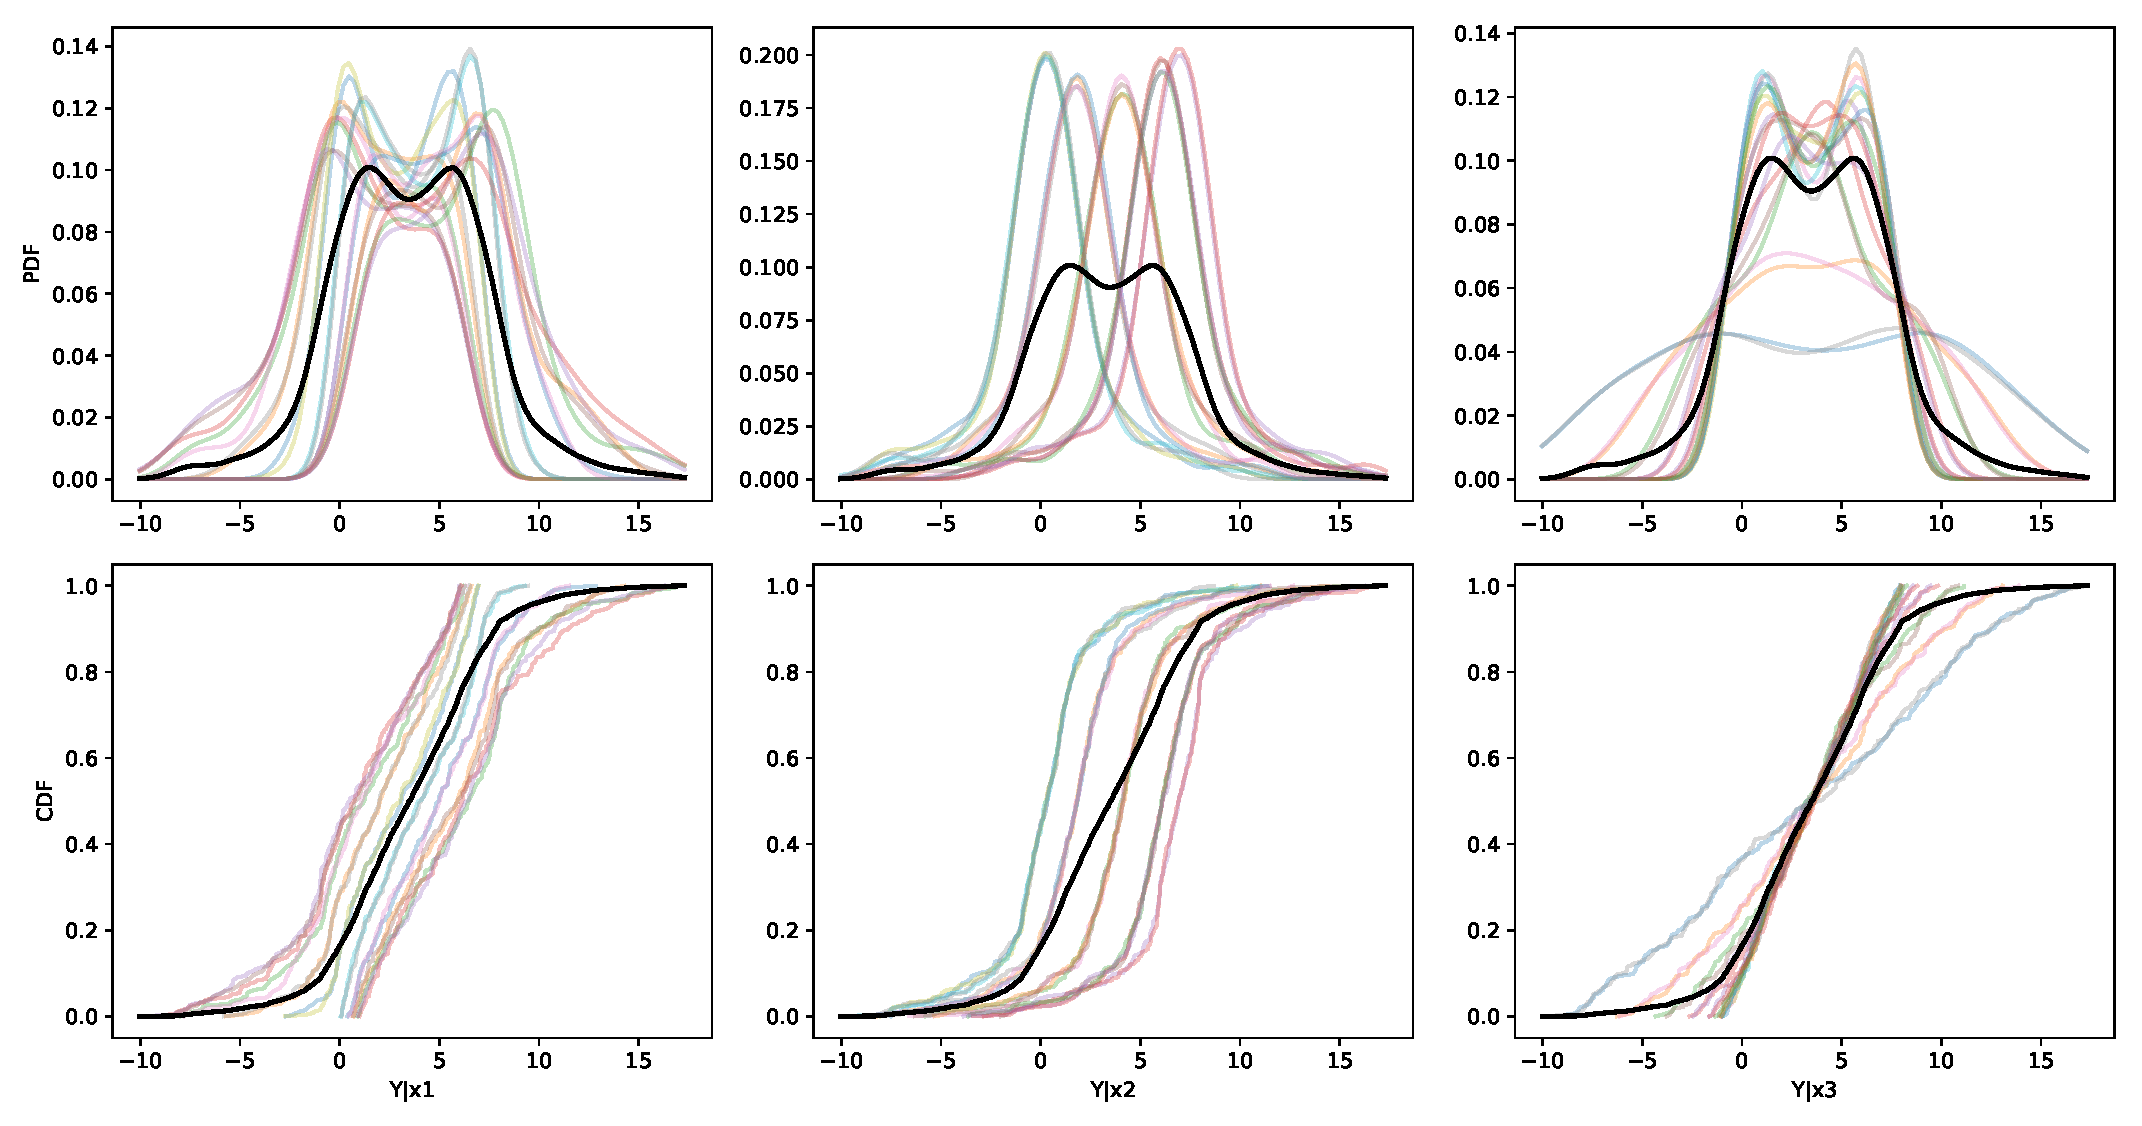
\includegraphics[width=\linewidth,keepaspectratio]{fig/literature/moment_independent-ishigami.pdf}
\caption{Moment independent SA on the \emph{Ishigami} function.}
\label{fig:moment_sa}
\end{figure}

Another visual approach is found with the Cumulative Sums Of NOrmalized Reordered Output method (CUSUNORO)~\cite{Plischke2012}. The output is normalized and ordered in function of a given parameter. Then, its cumulative sum vector is computed. In other words, this corresponds to the conditional ECDF after normalization. Here as well, the more the curve is far from the unconditional ECDF (a flat line after normalization), the more the output is sensitive to the parameter---see~\cref{fig:cusunoro}.

\begin{figure}[!h]
\centering
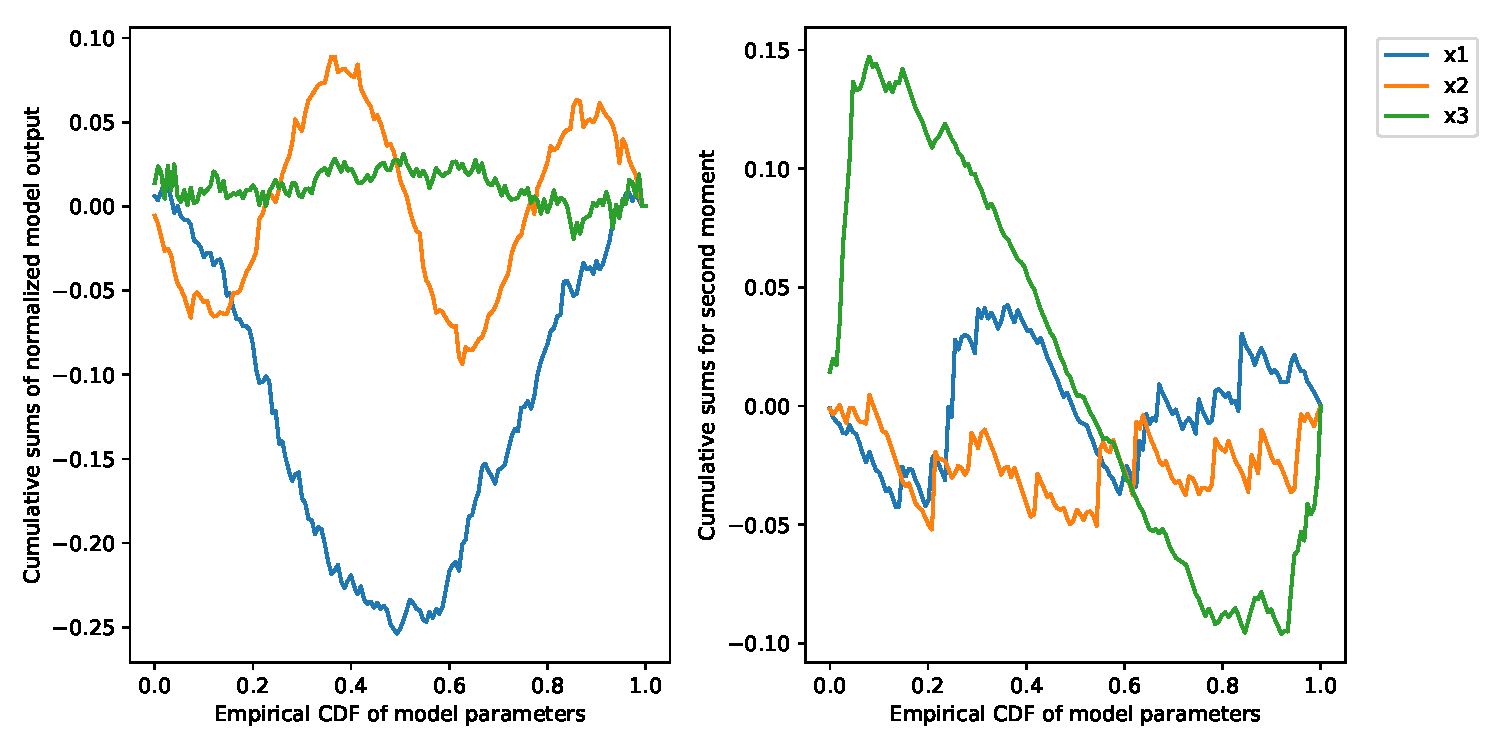
\includegraphics[width=0.8\linewidth,keepaspectratio]{fig/literature/cusunoro-ishigami.pdf}
\caption{CUSUNORO on the \emph{Ishigami} function.}
\label{fig:cusunoro}
\end{figure}


\section{Surrogate Models}\label{sec:surrogate}

\lettrine{C}{lassical} UQ methods, based on the Monte-Carlo approach, require a large number of experiments~\citep{iooss2010,iooss2016,lamboni2011,lemaitreknio2010,saltelli2007,storlie2009}, which quickly go beyond the limits of available resources (CPU cost, budget). In the following, numerical smulations are considered and especially CFD simulations. These limits are especially true when it comes to large dimensional problems, both with respect to the domain discretization and to the number of uncertain input parameters. The cost of the UQ study can, however, be significantly reduced when the CFD code is replaced by a surrogate model which is formulated in a parameter space and which is fast to evaluate for any set of uncertain variables~\cite{martin2005}.

Formulating the surrogate model relies on a limited number of forward model integrations referred to as the DoE. Several surrogate models are found in the literature, among whom generalized linear models, polynomial models, splines, Polynomial Chaos (PC) expansions, artificial neural networks or Gaussian Process (GP) models. In this work, two types of surrogate models are used to approximate the behaviour of forward models. PC expansion on the one hand, GP regression on the other hand. 

PC approach has received much attention lately~\citep{dubreuil2014,sudret2008,xiu2010,xiu2002,Ciriello2013}. The PC surrogate model is formulated as a polynomial expansion, in which the basis is defined according to the distribution of the uncertain inputs $\mathbf{x}$ and the coefficients relate to the statistics of the output $\mathbf{Y}$. The coefficients are computed so as to fit the training set $(\mathbf{X}, \mathcal{Y})$, either using regression or spectral projection methods. The merits of PC surrogates were demonstrated in various fields, e.g.~structural mechanics~\citep{dubreuil2014,berveiller2005}, CFD~\citep{hosder2006,lucor2007,saad2007phd}, hydrology~\citep{deman2015}, hydraulics~\citep{ge2008,elmocaydphd}, wildfires~\citep{rochoux2014}. A complementary approach between PC and EnKF was presented in~\citet{lixiu2009} and tested in the framework of wildfire behaviour forecasting in~\citet{rochoux2014}. A PC surrogate was used in place of the forward model to estimate the Kalman gain and thereby design a cost-effective EnKF inferring new estimates of the input parameters (e.g.~biomass moisture and fuel aspect ratio) reducing bias in the fire front location prediction. The resulting algorithm achieved convergence in spite of the non-linear surface response, showing promising results for environmental risk monitoring. 

GP that are strongly related to Kriging in geostatistics also are of increasing interest~\citep{rasmussen2006,legratiet2017,lockwood2012,marrel2015}. The GP formalism treats the forward model response as a realization of a Gaussian stochastic process indexed by $\mathbf{x}$ and fully characterized with mean and covariance functions conditioned by the training set $(\mathbf{X}, \mathcal{Y})$. The GP surrogate is built first, by defining a covariance kernel function between output values and a trend function and then, by estimating the hyperparameters (e.g.~variance, characteristic length scale) that provide a good fit to the training set. GP surrogates were introduced in the context of SA for estimating \emph{Sobol'} indices~\citep{oakley2004,marrel2009,legratiet2014}. In an industrial context---which is the case here---, some benefits of this method are:\textit{(i)} it does not require any prior knowledge on the probability distribution of the uncertainties on the input parameters ; \textit{(ii)} it does not need a specific sampling of the parameter space which could lead to \textit{curse-of-dimensionality} or mis-evaluation of the space ; and \textit{(iii)} it provides an estimation of the predictive error.

PC and GP surrogate models have recently been compared for UQ and SA studies~\citep{legratiet2017,owen2015,schoebi2015}. \citet{owen2015} evaluated the performance of each type of surrogate in terms of output mean, variance and PDF estimation. \citet{legratiet2017} compared \emph{Sobol'} indices with applications in structural mechanics; for a given size of the training set, PC and GP surrogate models were found to feature a similar predictive quality---with respect to the predictive coefficient $Q_2$, also called Nash-Sutcliffe model efficiency coefficient, which is equivalent to the coefficient of determination $R^2$ for residuals' prediction~\citep{krause2005} (see~\cref{sec:validation}). \citet{legratiet2017} also emphasized that the ranking between PC and GP approaches remains problem-dependent.

Before going further, let us clarify the nature of the forward model. The ensemble $\mathcal{Y}$ constitute a set of observed QoI. Each element can either be a scalar or a vectorial---or functional---QoI. When considering scalar QoI, a global physical parameter such as the mean temperature for instance, a single surrogate model mapping $Y^{(i)} := \mathcal{M}(\mathbf{x}^{(i)})$ can be constructed. In case of a multidimensional output the mapping comes to $\mathbf{Y}^{(i)} := \mathcal{M}(\mathbf{x}^{(i)})$. One can consider independent surrogate for each element but the computational cost can rapidly become intractable. Moreover, the elements of the vectorial QoI can be correlated. A classical solution is found through the use of a Proper Orthogonal Decomposition (POD)~\cite{anindyachatterjee2000}. By performing a POD on the QoI, each mode being orthogonal, they can be treated as independent and then a surrogate can be built on a reduced space. In~\cite{braconnier2011,margheri2016}, this method was used to reduce the computational cost and conserve the spatial/temporal correlation of the QoI.

Considering the general case of a functional QoI, the common idea of PC and GP approaches is to design for each element (with or without considering a POD) $a \in \{a_1, \cdots, a_M\}$ a surrogate with a weighted finite sum of basis functions:
\begin{align}
\widehat{Y}_a\left(\mathbf{x}\right) = \displaystyle\sum_{i = 0}^{r}\,\gamma_{a,i}\,\Psi_{i}\left(\mathbf{x}\right),
\label{eq:SurrogateForm}
\end{align}
where the coefficients $\gamma_{a,i}$ and the basis functions $\Psi_i$ are calibrated by the training set $\mathbf{X}^{N_s}$. The main difference between PC (Sect.~\ref{sec:PC}) and GP (Sect.~\ref{sec:GP}) approaches stands in the nature of these models: GP interpolates the training points and captures local variations, while PC is a regression method focusing on the global behaviour of the model. Basis functions and calibration methods also differ between these two approaches.

\Cref{sec:POD} present the POD while \cref{sec:PC} and \cref{sec:GP} respectively define the PC and the GP surrogate methods.

%For PC expansion, the maximum order of the decomposition and the basis functions are first chosen, then a spectral projection strategy is implemented to compute the decomposition coefficients in the polynomial basis. The GP strategy is two-fold: the first step consists in transforming the sampled output space to an orthogonal one, eventually reducing its dimension; the second step consists in interpolating with a GP approach the principal components of this new space to express water level in the basis for any friction and discharge values. It should be noted that the GP model could be replaced by any other interpolator. 

\subsection{Snapshot method}\label{sec:POD}

The key idea of the snapshot method~\citep{sirovich1987} is to achieve a POD of the centred snapshot matrix $\mathcal{Y} \in \mathbb{M}_{M,N}(\mathbb{R})$, which gathers the discretized QoI for the $N_{s}$ snapshots, from which the sample mean is subtracted. For simplicity purpose, the QoI anomaly element $a$ is denoted $y$ in the following. Thus, $\mathcal{Y} = \left(y_{a_i}^{(j)}\right)_{1\leq i \leq M \atop 1\leq j \leq N_{s}}$. The snapshots correspond to the column vectors; the $k$th snapshot of size $M$ is denoted by $\mathbf{y}^{(k)}$.

Based on many observations of a random vector, the POD gives the orthogonal directions of largest variances (or modes) in the probabilistic vector space in order to reduce the vector space dimension~\citep{chatterjee2000}. Note that for simplicity purpose, the adjective {\it centred} is dropped in the following when referring to the centred snapshot matrix $\mathcal{Y}$.

The POD of the snapshot covariance matrix $\mathbf{C} = N_{s}^{-1}\,\mathcal{Y}^{\mathrm{T}}\,\mathcal{Y}\in \mathbb{M}_{N_{s}}(\mathbb{R})$ is equivalent to the Singular Value Decomposition (SVD) of the snapshot matrix $\mathcal{Y}$:
\begin{align}
\mathcal{Y} = \mathbf{U}\,\mathbf{\Lambda}\,\mathbf{V}^{\mathrm{T}} = \displaystyle\sum_{k = 1}^{r_{p}}\,\lambda_k\,\mathbf{u}_k\,\mathbf{v}_k^{\mathrm{T}},
\end{align} 
where $\mathbf{U} \in \mathbb{M}_M(\mathbb{R})$ is an orthogonal matrix diagonalizing $\mathcal{Y}\mathcal{Y}^{\mathrm{T}}$ ($\mathbf{u}_k$, the $k$th column of $\mathbf{U}$, is a left singular vector of $\mathcal{Y}$), where $\mathcal{V} \in \mathbb{M}_N(\mathbb{R})$ is an orthogonal matrix diagonalizing $\mathcal{Y}^{\mathrm{T}}\mathbf{Y}$ ($\mathbf{v}_k$, the $k$th column of $\mathbf{V}$, is a right singular vector of $\mathcal{Y}$), and where $\mathbf{\Lambda} \in \mathbb{M}_{M,N_{s}}(\mathbb{R})$ is a rectangular diagonal matrix including $r_{p}=\min(M,N_{s})$ singular values on its diagonal. The singular values $\lbrace \lambda_k \rbrace_{1 \leq k \leq r_{p}}$ are the square roots of the eigenvalues of $\mathbf{C}$. 
Note that in this study, we do not reduce further the rank of the snapshot matrix $\mathcal{Y}$. %Since the number of stations ($M = 14$) is lower than the size of the training set $N$, the rank of $\mathbf{Y}$ is here $r_{p} = M$.

For a given element $a$, any snapshot $h_a(\mathbf{x}^{(k)})$ can then be retrieved as a linear combination of $r_{p}$ modes $\{\Psi_i\}_{1\leq i \leq r_p}$:
\begin{align}\label{eq:gppod}
y_a(\mathbf{x}^{(k)}) 
= (\mathbf{U}\,\mathbf{\Lambda}\,\mathbf{V}^{\mathrm{T}})_{ak} 
= U_{a:}(\mathbf{\Lambda}\,\mathbf{V}^T)_{:k}=\sum_{i=1}^{r_{p}}\,\gamma_{a,i}\,\Psi_i(\mathbf{x}^{(k)}),
\end{align}
where for any $i\in\{1,\ldots,M\}$, $\gamma_{a,i}:=U_{a,i}$ and $\Psi_i(\mathbf{x}^{(k)}):=(\boldsymbol{\Lambda}\mathbf{V}^T)_{i,k}$. 
%
%In the present study, the size of the state vector $M$ is smaller than the size of the training set $N$, implying that there are $r_p = M$ non-zero singular values. This is usually not the case, but this does not change the methodology. As the objective is to compare PC and pGP and as there is a limited number of stations $M$, all modes are kept to avoid the loss of information, there is no need to reduce the rank of the singular matrix. Note that when moving to 2-D or 3-D cases (beyond the scope of the present work), the size of the state vector could be of the order of thousands components, making dimension reduction necessary. 


%----Polynomial Chaos
\subsection{Polynomial Chaos (PC) surrogate model}\label{sec:PC}

The algorithm to build the PC surrogate proceeds as follows:
\begin{enumerate}
\item choose the polynomial basis $\lbrace\Psi_{i}\rbrace_{i\geq 0}$ according to the assumed PDF of the inputs $\mathbf{x}$,
\item choose the total polynomial degree $P$ according to the complexity of the physical processes,
\item truncate the expansion to $r_{\text{pc}}$ terms to keep the predominant information given by the forward model using standard truncation strategy ($r_{\text{pc}}$ depends on $d$ and $P$),
\item apply spectral projection strategy (i.e.~Gaussian quadrature rule) to compute the coefficients $\lbrace\gamma_{a,i}\rbrace_{i\in\mathbb{N}^d\atop|i|\leq P}$ for each element $a$ (can use a POD or not) using $N_{s} = (P+1)^{d}$ snapshots,
\item formulate the surrogate model $\mathcal{M}_{\text{pc}}$ at each element $a$, which can be evaluated for any new pair of parameters $\mathbf{x}^*$.
\end{enumerate}
Note that we use standard truncation and projection strategies presented in~\cite{lemaitreknio2010} and \cite{xiu2010}.

\subsubsection{Polynomial basis}

Each component of the random vector $\mathbf{x}$ defined in the input physical space is standardized and noted $\boldsymbol{\zeta}$ in the following way: $\zeta_i=\frac{x_i-\mu_i}{\sigma_i}$ where $\mu_i=N_{s}^{-1}\sum_{k=1}^{N_{s}}x_i^{(k)}$ and $\sigma_i=\sqrt{(N_{s}-1)^{-1}\sum_{k=1}^{N_{s}}\left(x_i^{(k)}-\mu_i\right)^2}$. 

%Assuming that the SWE solution is of finite variance, each component $h_a$ of the water level vector $\mathbf{h}$ can be considered as a random variable for which there exists a polynomial expansion of the form~\eqref{eq:SurrogateForm} that represents how the water level $h_a$ varies according to changes in $Q$ and $K_{s_3}$. 

$y_a$ is projected onto a stochastic space spanned by the orthonormal polynomial functions $\lbrace\Psi_{i}\rbrace_{i\geq 0}$. These functions are orthonormal with respect to the joint density $\rho(\boldsymbol{\zeta})$, i.e.
\begin{align}
\int_{Z}\,\Psi_i(\boldsymbol{\zeta})\,\Psi_j(\boldsymbol{\zeta})\,\rho(\boldsymbol{\zeta})\,\mathrm{d}\boldsymbol{\zeta} = \delta_{ij},
\label{eq:pc_innerproduct}
\end{align}
with $\delta_{ij}$ the Kronecker delta function and $Z \subseteq \mathbb{R}^d$ the space in which $\boldsymbol{\zeta}$ evolves.

In practice, the orthonormal basis is built using the tensor product of 1-D polynomial functions: $\Psi_i=\Psi_{i,1}\ldots\Psi_{i,d}$ where $i$ is the multi-index $(i_1,\ldots,i_d)\in\{0,1,\cdots,P\}^d$. The choice for the basis functions depends on the probability measure of the random variables. According to Askey's scheme, the Hermite polynomials form the optimal basis for random variables following the standard Gaussian distribution, and the Legendre polynomials are the counterpart for the standard uniform distribution~\citep{xiu2002}. 

\subsubsection{Truncation Strategy}

In practice, the sum in Eq.~\eqref{eq:SurrogateForm} is truncated to a finite number of terms $r_{\text{pc}}$. Using a standard truncation strategy $r_{\text{pc}}$ is constrained by the number of random variables $d$ and by the total polynomial degree $P$ as:
\begin{align}
r_{\text{pc}} = \frac{(d + P)!}{d!\,P!},
\label{eq:pc_order}
\end{align}
meaning that all polynomials involving the $d$ random variables of total degree less or equal to $P$ are retained in the PC expansion. The PC approximated the QoI at each element $y_{\text{pc}}(a)$ is formulated as:
\begin{align}
\widehat{y}_{\text{pc},a}(\mathbf{x}) := \mathcal{M}_{\text{pc},a}(\boldsymbol{\zeta}) = \displaystyle\sum_{i\in\mathbb{N}^d\atop|i|\leq P}\,\gamma_{a,i}\,\Psi_i\left(\boldsymbol{\zeta}\right).
\label{eq:SurrogatePC}
\end{align}
Note that for small $d$, advanced truncation strategies that consist in eliminating high-order interaction terms or using sparse structure~\citep{blatman2009phd,migliorati2013} are not necessary.

\subsubsection{Spectral projection strategy}

We focus here on non-intrusive approaches to numerically compute the coefficients $\lbrace\gamma_{a,i}\rbrace_{i\in\mathbb{N}^d\atop |i|<P}$  in Eq.~\eqref{eq:SurrogatePC} using $N_{s}$ snapshots from $\mathbf{X}^{N_s}$. The spectral projection relies on the orthonormality property of the polynomial basis. The $i$th coefficient $\gamma_{a,i}$ is computed using Gaussian quadrature as:
\begin{align}
\gamma_{a,i} = <y_a,\Psi_i> \,\cong\,\displaystyle\sum_{k = 1}^{N_{s}}\,y_a^{(k)}\,\Psi_i(\boldsymbol{\zeta}^{(k)})\,w^{(k)},
\label{eq:pc_quadrature}
\end{align}
where $\mathbf{y}^{(k)} = \mathcal{M}(\mathbf{x}^{(k)})$ is the snapshot corresponding to the $k$th quadrature root $\mathbf{x}^{(k)}$ of $\Psi_i$ (in the physical space), and where $w^{k}$ is the weight associated with $\mathbf{x}^{(k)}$. $(P+1)$ is the number of quadrature roots required in each uncertain direction to ensure an accurate calculation of the integral $<y_a,\Psi_i>$. Hence, $N_{s} = (P+1)^2$.


%----Gaussian process
\subsection{Gaussian Process (GP) surrogate}\label{sec:GP}

The algorithm to build a Gaussian Process surrogate proceeds as follows:
\begin{enumerate}
\item choose the size of the training set $N_{s}$,
\item draw $N_{s}$ samples (or snapshots) in the input random space $\mathbf{x}$,
%\item formulate the centred snapshot matrix $\mathcal{Y}$ from the $N_{s}$ snapshots,
%\item achieve a POD on $\mathbf{Y}$ using the snapshot method to derive the basis vectors $\lbrace\Psi_{i}\rbrace$ and the corresponding coefficients $\lbrace\gamma_{a,i}\rbrace$ (any snapshot can be expressed as a linear combination of the basis vectors and coefficients),
%\item replace each basis vector $\lbrace\Psi_i\rbrace$ associated to the $N_{s}$ snapshots by a basis function via Gaussian Process regression for any $\mathbf{x}^*$, 
\item formulate the surrogate model $\mathcal{M}_{\text{gp}}$ for the QoI at each element $a$ (can use a POD or not), which can be evaluated for any $\mathbf{x}^*$.
\end{enumerate}

\subsubsection{Regression Procedure}\label{sec:regression}

%In this case, the random variable being the POD coefficients computed for each random input vector $\mathbf{x}$ of $N_s$: $f(\mathbf{x}) = (\mathbf{\Sigma}_{k} \mathbf{V}^T_{k})_{\mathbf{x}}$. A new prediction consists in a new column of $\mathbf{\Sigma}_{k} \mathbf{V}^T_{k}$.

A Gaussian Process (GP) is a collection of random variables which have a joint Gaussian distribution~\cite{rasmussen2006}. GP is equivalent to \textit{Kriging}~\cite{krige1989}. A \textit{Gaussian Process} is described by its mean $\mu(\mathbf{x})$ and covariance $k(\mathbf{x},\mathbf{x}')$---where $\mathbf{x}, \mathbf{x}'$ are different sets of inputs

\begin{align}
Y_a(\mathbf{x})&\sim \mathcal{GP}(\mu(\mathbf{x}), k(\mathbf{x},\mathbf{x}')), \;\text{with} \\
m(\mathbf{x}) &= \mathbb{E}\left[ Y_a(\mathbf{x})  \right], \nonumber \\
k(\mathbf{x},\mathbf{x}') &= \mathbb{E}\left[ (Y_a(\mathbf{x}) -\mu(\mathbf{x}))(Y_a(\mathbf{x}')-\mu(\mathbf{x}')) \right] \nonumber.
\end{align}

Here the covariance function $k$ (or kernel) is chosen as a squared exponential
\begin{align} 
K = k(\mathbf{x}, \mathbf{x}') = \sqrt{\pi} \; \sigma_\mathbf{x}^2 \exp\left(-\frac{\|\mathbf{x} - \mathbf{x}'\|^2}{2\,\ell_i^2}\right), 
\end{align}
where $l$ is a length scale that describes the trend in the data and $\sigma_\mathbf{x}$ is the variance of the output signal. Squared exponential kernel leads to satisfying results but other kernel functions could have been considered, such as a decreasing exponential one or a \emph{Matérn} one -- with their associated hyper-parameters. The choice of the kernel is still an open problem and can be mitigated using the available information on the problem. The square exponential kernel leads to very smooth, thus stable results. Furthermore, it implies that the model is exact at sample points; it does not introduce any other strong assumptions, hence its wide usage among practitioners.

Then the GP model consists of a regression providing an interpolation $\mathcal{M}_{\text{gp}}$ for a new set of input parameters $\mathbf{x^{*}}$:
\begin{align}
\mathcal{M}_{\text{gp}_{a}}(\mathbf{x}^*)&=\bar{Y_{a}}(\mathbf{x}^*) =  \sum_{i = 1}^{N_s}\alpha_i k (\mathbf{x}^i, \mathbf{x}^*), \;\text{with} \\
\mathbf{\alpha} &= (K + \sigma_n^2 I)^{-1}\mathcal{Y}_a, \nonumber
\end{align}
where $\bar{Y_a}$ is the mean realization, $\mathbf{x}^i$ the \textit{i-th} set of parameters, $\mathcal{Y}_{a}$ the snapshot matrix considering element $a$ and $\sigma_n$ is the nugget effect that prevent ill-conditioning issues for the matrix $K$. Indeed, it is the mean realization of the conditioned process considering an artificial noisy observation which gives the prediction. The learning phase of the GP consists in selecting $l$, $\sigma_n$ and $\sigma_\mathbf{x}$ so that $Y_a$ passes through or close to the dataset points. These hyperparameters are optimized by maximizing the log likelihood applied to the data set $\mathcal{Y}_a$ using a basin hopping technique~\citep{wales1997}. A key advantage of this predictor is that it provides an inference about its prediction variance
\begin{align}
\mathbb{V}[Y_{a}(\mathbf{x}^*)] = k(\mathbf{x}^*, \mathbf{x}^*)-\mathbf{k}(\mathbf{x}^*)^T(K + \sigma_n^2 I)^{-1}\mathbf{k}(\mathbf{x}^*).
\end{align}
The regression methodology is shown in~\cref{fig:gp_prior-post}. On \cref{fig:gp_prior-post}(a), the GP is sampled on the input parameter space. In this case, a GP with zero mean and unit variance is used. It means that for each $x^i$, the QoI is estimated as a Gaussian process of zero mean and unit variance. Thus along the parameter $x_{k}$, the GP is defined as an infinite collection of GPs. The link between each GP is assured through the correlation matrix defined by the kernel. Once some observations are added---see~\cref{fig:gp_prior-post}(b)---, the GP is conditioned so that each realization of the GP passes through the observations. This intrinsic property of the GP can be relaxed by changing the diagonal of the correlation matrix. This can be used to take into account some noise in the data for instance. Moreover, the matrix can be adapted per observation if the variance of the noise is known to be different---heteroscedastic noise.

As said beforehand, the hyperparameters are choosen as to maximize the marginal log likelihood. It is the integral of the likelihood times the prior marginalized over the function values:
\begin{align}
p(y|x) = \int p(y|\mathbf{f}, x)p(\mathbf{f}|x)d\mathbf{f}.
\end{align}
\noindent In other words, maximizing this quantity will tend to reduce the confidence interval between each points. It is to be noted that along each direction of the parameters space, having different set of hyperparameters  is possible so that anisotropy can be taken into account.

\begin{figure}[!h]
\centering
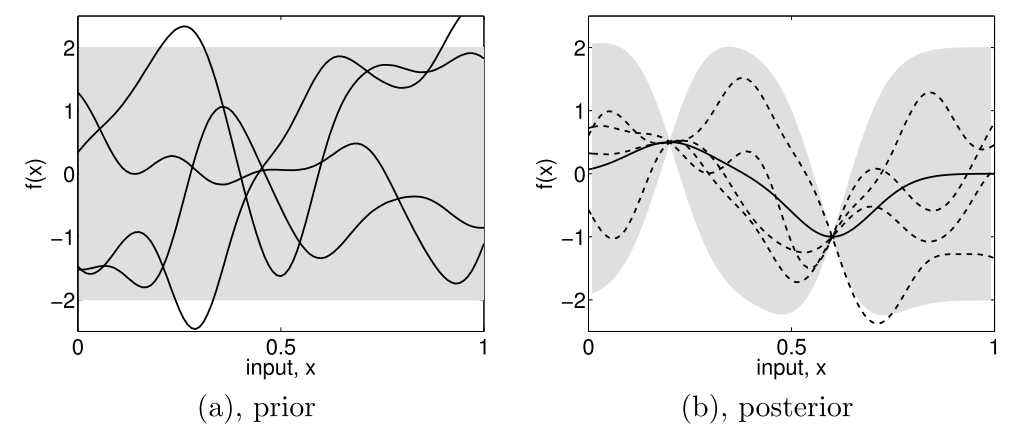
\includegraphics[width=0.9\linewidth,keepaspectratio]{fig/literature/rasmussenGP.png}
\caption{Visualization of 4 Gaussian processes: \textbf{a} represents a sampling of the GP while in \textbf{b} these functions have been conditioned on two points. Shaded regions represent twice the standard deviation of the GPs. Source: \cite{rasmussen2006}.}
\label{fig:gp_prior-post}
\end{figure}



\subsection{Model Validation}\label{sec:validation}

An important step after having constructed a surrogate model is to access its validity. There are lots of ways to do this and the common step is to compare the prediction of the model at a given point with its actual value. Depending on the number of simulation that can be afforded, extra validation simulation not used for constructing the model can be performed. On the other hand, the same dataset can be used.

\begin{figure}[!h]
\centering
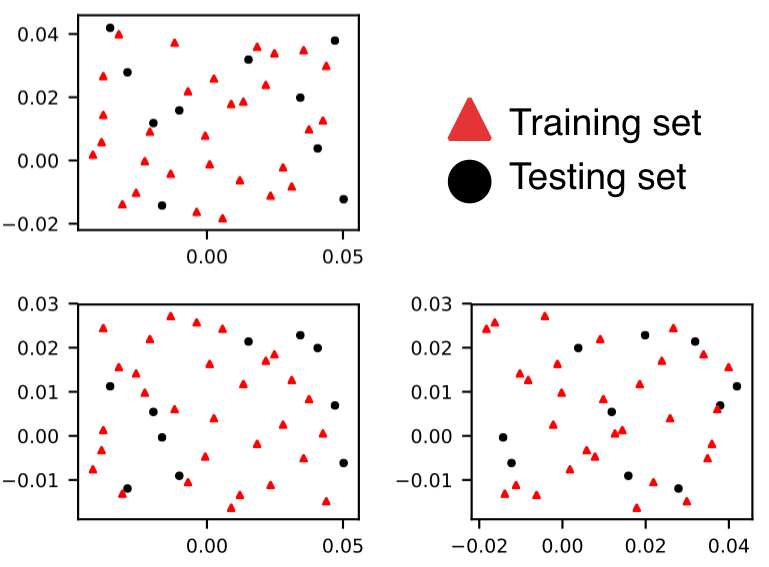
\includegraphics[width=0.6\linewidth,keepaspectratio]{fig/literature/validation_set.png}
\caption{3-dimensional parameter space canonical visualization of training (triangles) and validation (circles) sets.}
\label{fig:validation}
\end{figure}

\subsubsection{Mean Square Error and alike}
Various metrics are used to compare the results of a known sample over the result of a prediction from a model. The Mean Square Error (MSE) basically computes the sum of the square differences. Taking its root allows to conserve the dimensionality of the QoI
\begin{align}
\text{RMSE} = \sqrt{\frac{1}{N}\,
\displaystyle\sum_{i = 1}^{N}\,(Y_i - \hat{Y}_{i})^2}.
\end{align}
However, this method is not robust to outliers as one or two values can lead to large errors. Mean absolute error and median absolute error have a better behaviour toward this. In any case, the lower the error, the better the model.

\subsubsection{Coefficient of Determination: $R^2/Q_2$}
Another common indicator is the determination coefficient also called predictivity coefficient $Q_2$~\citep{marrel2009}. It is composed of both the mean square error and the variance of the output. It is a normalization of the MSE by the spread of the data. The variance normalization makes this indicator strictly lower than 1. This is handy for comparing models with each other as the QoI's units does not counts.
\begin{align} 
Q_{2} = 1 - \frac{\displaystyle\sum_{i = 1}^{N}\,\left(Y_i - \widehat{Y}_i\right)^2}{\displaystyle\sum_{i = 1}^{N}\,\left(Y_{i} - \overline{Y}_i\right)^2}.
\end{align}
A perfect model would have a $Q_2=1$. With a constant model, $\hat{Y}$ is equal to the mean leading to $Q_2=0$. Finally, $Q_2=0$ can be negative, meaning that the model is arbitrary worse than a constant model.

\subsubsection{Kolmogorov-Smirnov statistical test}

The Kolmogorov-Smirnov test is a classical method used to evaluate the similarity between PDF~\citep{clarke1992}. Let $T_F$ (resp. $T_G$) be a random variable with cumulative distribution function (CDF) $F$ (resp. $G$). Let $F_n$ (resp. $G_m$) be its empirical CDF built from $n$ (resp. $m$) independent realizations of $T_F$ (resp. $T_G$). Then, let us define the test statistics:
\begin{align}
D = \sup_{x} \lvert F_n(x) - G_m(x)\rvert.
\end{align}
The null hypothesis for the Kolmogorov-Smirnov statistical test supposes that $T_F$ and $T_G$ are identically distributed, i.e.~$F=G$. The Kolmogorov-Smirnov test leads us to reject this hypothesis with a type I error $\alpha\in]0,1[$ when:
\begin{align}
D > c(\alpha)\,\sqrt{\frac{n+m}{nm}}, \label{eq:nullhypothesis}
\end{align}
with $c(\alpha)$ a tabulated value found in the literature~\citep{smirnov1939}. Considering $\alpha = 0.05$ and $n = m = N$, the null hypothesis is rejected if $D > \numprint{6.082e-3}$.

\subsubsection{Graphical Quality Assessment}
An easy way to visualize the quality of the model is to plot a joint plot. Its construction is simple. For a given sample, there is an observed value of QoI, let's say 5 (\cref{fig:qq_plot}). Then for the same sample, we take the predicted value of QoI, here also 5. These two values are used to construct a scatter plot. Thus, if the model is perfect, predicted values are equal to observed values leading to a line on this graph. On the right figure, the model is not as good as on the left, so an observed value of 5 is linked to a predicted value of 0.

\begin{figure}[!h]
\centering
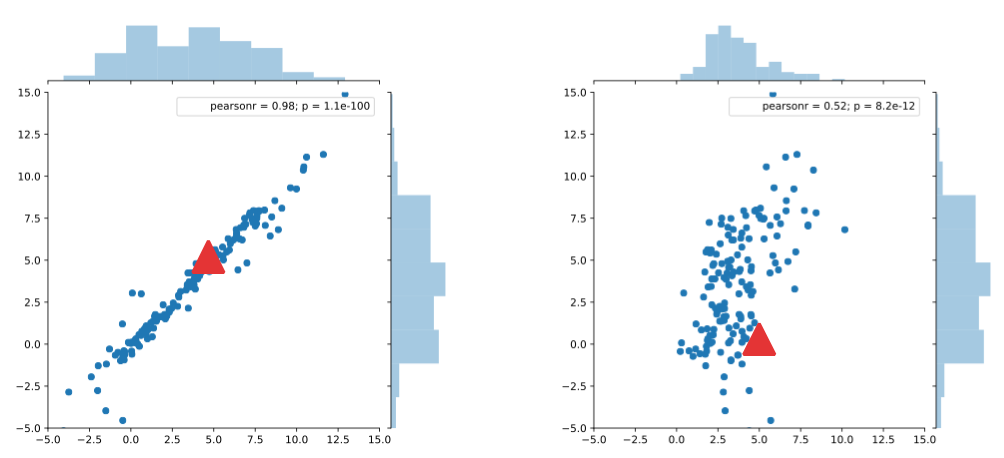
\includegraphics[width=0.9\linewidth,keepaspectratio]{fig/literature/qq_plot.png}
\caption{Joint plot. QoI function of the predicted QoI given a parameter set. The triangle represent an observed value of 5.}
\label{fig:qq_plot}
\end{figure}

\subsubsection{Holdout as opposed to \emph{K-fold} or cross validation}
To use these different metrics, we have to come up in some ways with a validation set. The classical approach is to use a validation set which is different than the training set. This holdout procedure requires to split the entire dataset into two disjoints datasets. There are no rules about the data sharing proportions. Things like the fitting time or the total number of samples leads to various splitting strategies.

Another method is to keep the same sample set for both training and validation. It is called cross-validation or \emph{K-fold}~\cite{kohavi1995}. In this case, $K$ different models are constructed on subsets of the dataset and the metrics are computed on the points that are not used during the fitting of these different models. For \emph{K-fold} to work optimally, it assumes that the model is fairly stable to these points removal. In~\cref{fig:k_fold}, $K=3$ which leads to 3 subsets of 6 points being created. These 6 points are used for training a model while the other 3 points are used for computing a metric. These operations are repeated 3 times and all metric's results are aggregated. A particular case is found with $K$ being equal to the number of sample. This is called \emph{leave-one-out}.

\begin{figure}[!h]
\centering

\includegraphics[width=0.6\linewidth,keepaspectratio]{fig/literature/k_fold.png}
\caption{Sketch of the \emph{K-fold} methodology. $K=3$ with $N=9$ which leads to 3 subsets of 6 points.}
\label{fig:k_fold}
\end{figure}


\section{Uncertainty Visualization}\label{sec:visu}
% Visualization issue
\lettrine{I}{n spite} of a large literature on UQ, the community has yet to propose efficient ways to visualize uncertainties. Indeed, to the author’s knowledge, there is no chapter dedicated to visualization in UQ reference books~\citep{saltelli2007,sullivan2015,handbookUQ}. This remains to be investigated, especially for Computational Fluid Dynamics (CFD) applications~\citep{Moreland2016} that involve complex fields of large dimensions. Classical ways of visualizing standard statistics can lead to misinterpretation~\citep{Anscombe1973}. The challenge for state-of-the-art visualization solutions stands in the dimension of the data. Assuming that the dimension of the data is limited (a set of scalars), for instance when dealing with input data, canonical subplots of subspaces are adapted. Parallel coordinate plots~\citep{Inselberg1985} or Kiviat plot (also referred to as spider plot)~\citep{Hackstadt1994} that are represented in~\Cref{fig:sketch_Kiviat-parallel} offer an interesting alternative and share the same idea of dedicating one input variable (noted $x_i$) per axis; Kiviat (right panel) plot being the equivalent to parallel coordinates (left panel) plot in polar coordinates. 
\begin{figure}[!h]
\centering
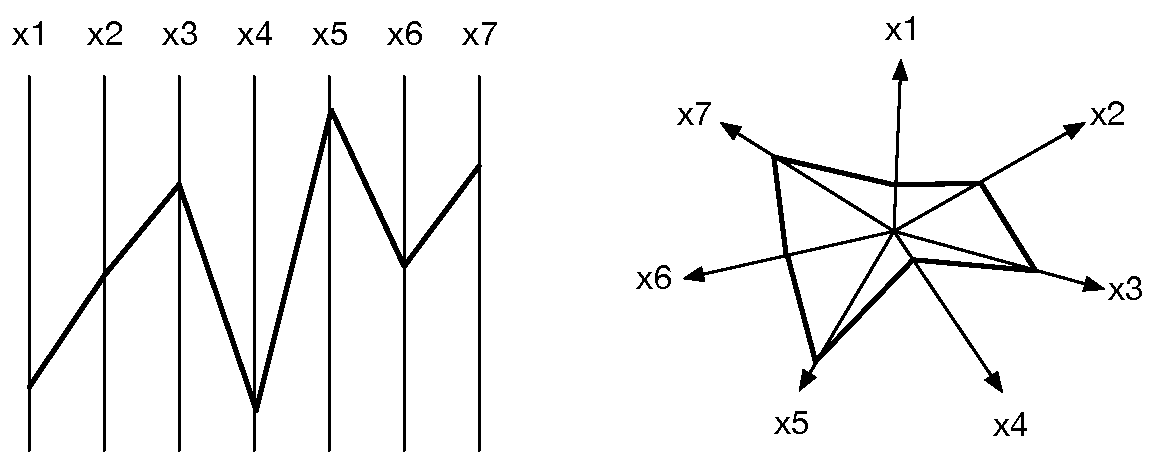
\includegraphics[width=0.8\linewidth,keepaspectratio]{fig/literature/parallel-kiviat.pdf}
\caption{Schematic representation of a parallel coordinate plot (\emph{left}) and a Kiviat plot (\emph{right}).}
\label{fig:sketch_Kiviat-parallel}
\end{figure}
% Outputs

When the dimension of the data increases, for instance when dealing with \emph{functional} output fields discretized in both space and time on fine meshes, advanced strategies should be proposed. Different strategies are found in the literature to visualize statistics on the response variable~\citep{Potter2012a,Brodlie2012,Bonneau2014}. Beyond deterministic simulation, moving on to ensemble-based approaches, the dimension of the data further increases.

A first approach is to look at each realization of the data set individually, in the output space with curves, maps or 3D-graphs. In the early work of Sir Francis Galton and its bean machine, the sampling process illustrated the demonstration of the central limit theorem stating that the binomial distribution approximates the normal distribution. The animated version of the sampling procedure is referred to as the Hypothetical Outcome Plots (HOPs) technique~\citep{Ehlschlaeger1997} and was generalized by~\citep{Hullman2015} for a set of scalars as presented in~\cref{fig:pattern_hop}.

HOPs consists in animating a succession of possible outcomes sampled from the data. It was proven to enable the exploration and the understanding of the dataset general characteristic, even for people lacking statistical background~\citep{Belia2005} with the possibility to visually grasp correlations in the outputs. 

\begin{figure}[!h]
\centering
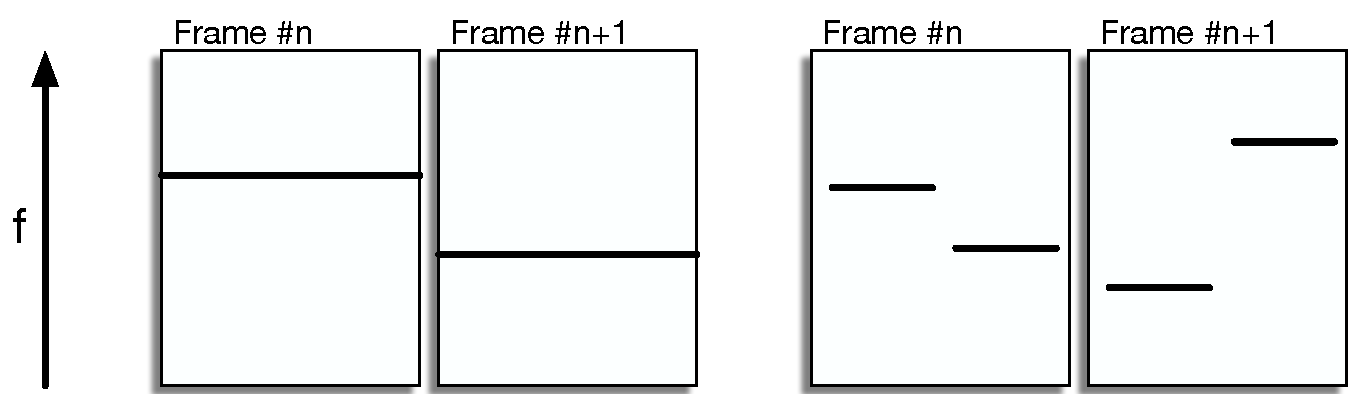
\includegraphics[width=0.8\linewidth,keepaspectratio]{fig/literature/pattern_hop.pdf}
\caption{Schematic representation of the HOPs method for single scalar output (\emph{left}) or multiple scalar outputs (\emph{right}).}
\label{fig:pattern_hop}
\end{figure}

Statistical moments and Probability Density Function (PDF) plot are common tool for visualizing uncertainties in the context of ensemble simulation as illustrated in~\cref{fig:pattern_pdf}. They are useful for risk analysis as the probability of exceeding a threshold is directly observable. \Cref{fig:pattern_pdf}(a) displays the PDF for a scalar response variable (noted $f$) where the mean, the mode and extreme probabilities can be observed. \Cref{fig:pattern_pdf}(b) displays the principal mode of the PDF (solid black line) for a functional response variable discretized in the $x-$direction. The PDF standard deviation (added/removed to/from the mean) is plotted in dashed lines. These curves are computed for each $x$ independently and they do not represent a possible solution of the numerical solver. The box plot in \Cref{fig:pattern_pdf}(c) provides similar information while diminishing the false illusion of median/mean curves. It should be noted that users usually have a better understanding of frequency~\citep{Gigerenzer1995} than of PDFs and that there is a  general misinterpretation of confidence intervals~\citep{Belia2005}.
%augmenting 1-dimensional \emph{boxplot} visualizations 
\begin{figure}[!h]
\centering
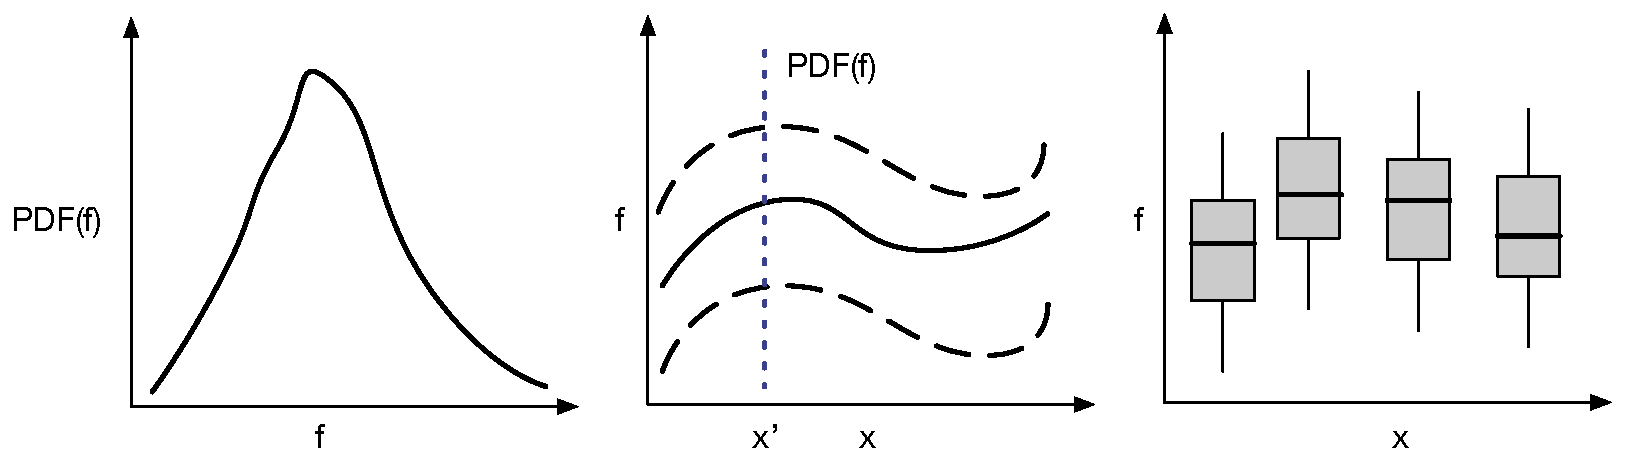
\includegraphics[width=\linewidth,keepaspectratio]{fig/literature/patterns_pdf.pdf}
\caption{Schematic representation of the PDF for a scalar output (\emph{left}), for a functional output (\emph{middle}) and with a boxplot solution (\emph{right}). The PDF mode is represented with a solid line, the standard deviation added/removed to/from the mean is represented with dashed lines.}
\label{fig:pattern_pdf}
\end{figure}

A complementary approach based on density criteria was proposed by~\citep{Hyndman2009,Sun2011}; it is noted HDR for Highest Density Region and represented in~\cref{fig:pattern_hdr}. It allows to depict some statistics (for instance median or outliers) taking into account the functional response variable as a whole and working in a reduced space spanned by the most significant directions of the output space. Within this reduced space, metrics for functional outputs are computed such as the distance to the median (blue curve) so that abnormal or outlier outputs (red and green curves) can be detected and quantiles can be estimated (blue envelope). Each curve represents either a realization within the data set or an additional realization sampled in the reduced space; thus functional characteristics such as spatial or temporal correlation are preserved.  From~\citep{Popelin2013,Ribes2015}, the HDR method is more robust to outlier detection than other methods such as functional boxplot~\citep{Sun2011,Whitaker2013}.

\begin{figure}[!h]
\centering
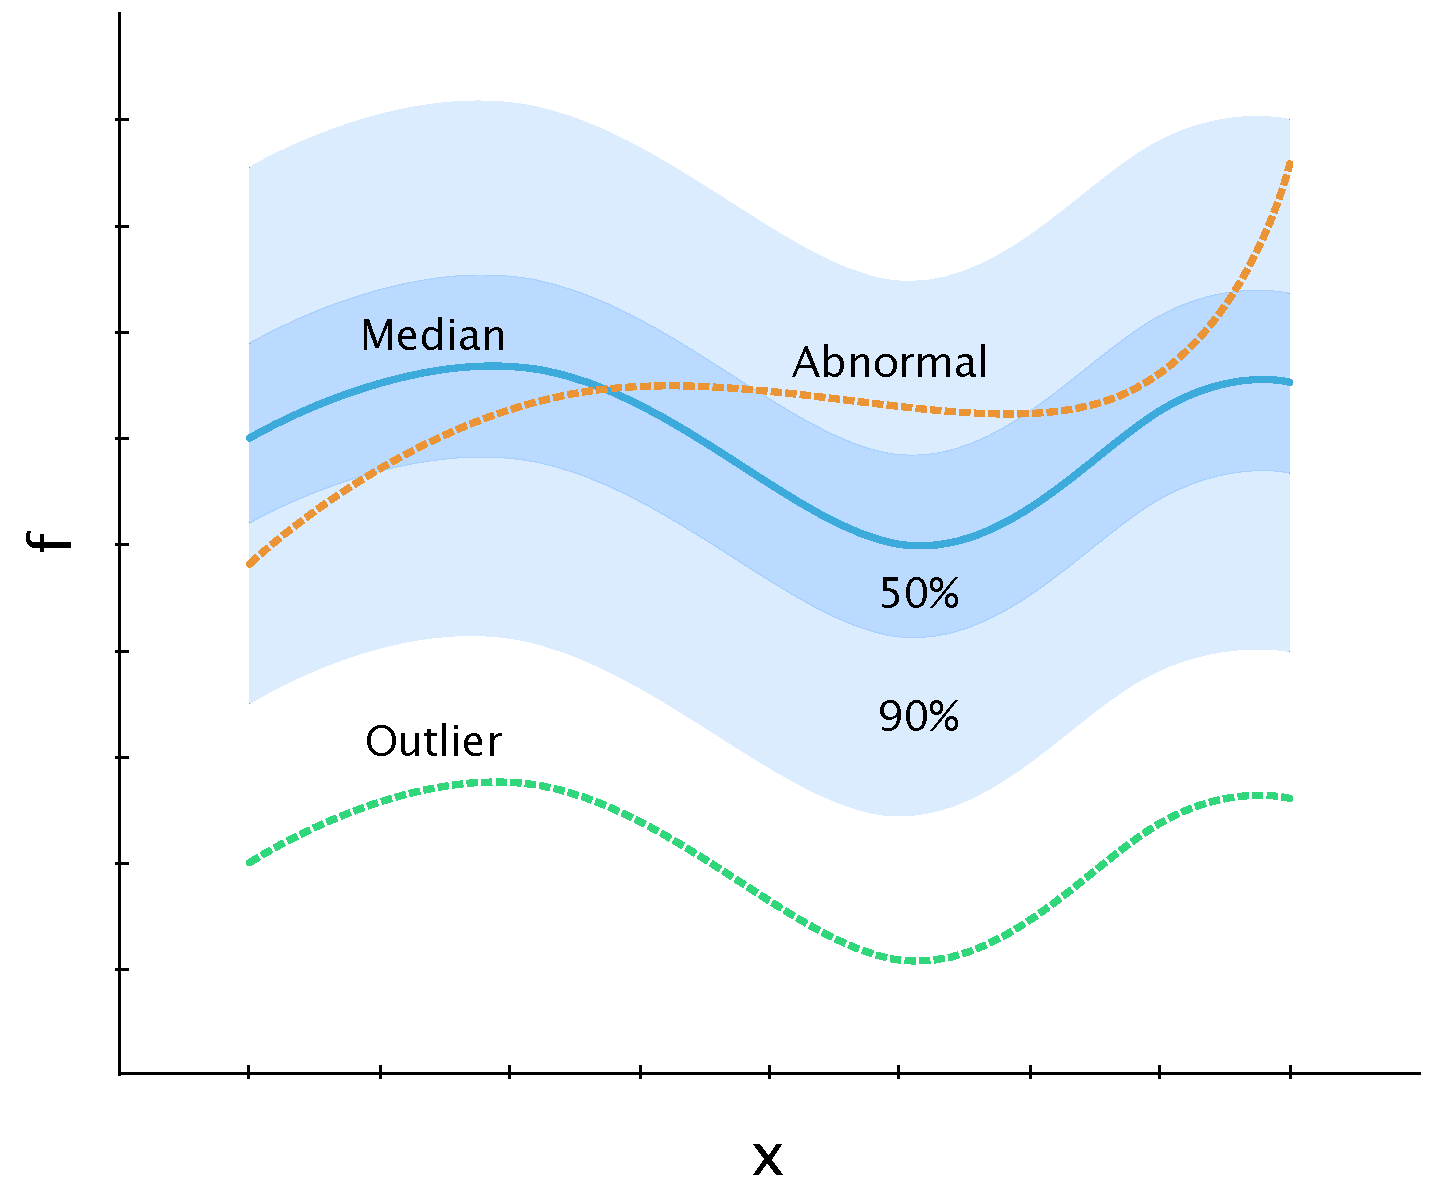
\includegraphics[width=0.6\linewidth,keepaspectratio]{fig/literature/pattern_hdr.pdf}
\caption{Schematic representation of data set functional realizations characterized with HDR metrics. The median is represented by the solid blue line, the abnormal and outliers are represented by the red and green lines and the 50\% and 90\% quantiles are represented by blue shaded envelopes.}
\label{fig:pattern_hdr}
\end{figure}

\subsection{Highest Density Region}
\label{sec:HDR}

The dataset output is considered as a matrix where each line corresponds to a realization. This matrix is decomposed by POD. The modes are ordered by decreasing importance in terms of contribution to the variance and only a finite number of modes are kept. In this reduced space, the functional dataset of large dimension is conveniently represented by a limited number of scalars mapped onto most significant directions that maximizes the variance of the response variable. Within this reduced space, the classification of different patterns or the computation of metrics is eased~\citep{Ren2017}. Hence, within this reduced space, the median realization corresponds to the HDR location. The distance to this point is computed in the modal space; the farther a point is from the HDR, the less probable is the realization.

A multivariate KDE (see~\cref{sec:up}) technique is used to estimate the PDF $\hat{f}(\mathbf{x_r})$ of this multivariate space. From this KDE, the HDR reads
\begin{align}
R_\alpha = {x_r: \hat{f}(\mathbf{x_r}) \geq f_{\alpha}},
\end{align}
\noindent with $f_{\alpha}$ such that $\int_{R_\alpha} \hat{f}(\mathbf{x_r}) d x_r = 1 - \alpha$. The region has a probability of containing $1-\alpha$ points that verify the highest density estimate. Thus the median curve is defined as the inverse transform---from the reduced space into the original space---of $\arg \sup \hat{f}(\mathbf{x_r})$. Also 50\% and 90\% highest density regions are computed---with respectively $\alpha=0.5$ and $\alpha=0.1$.

Except if the response variable of the system of interest is chaotic under the perturbation of its input parameters, the POD is expected to drastically reduce the dimensionality of the problem. Furthermore, as the system's response variable is also expected to oscillate around some modes, the points in the reduced space are likely to be relatively clustered around the modes. This mitigates the difficulty of the density estimation procedure.

\begin{figure*}[!h]               
\centering
\subfloat[]{
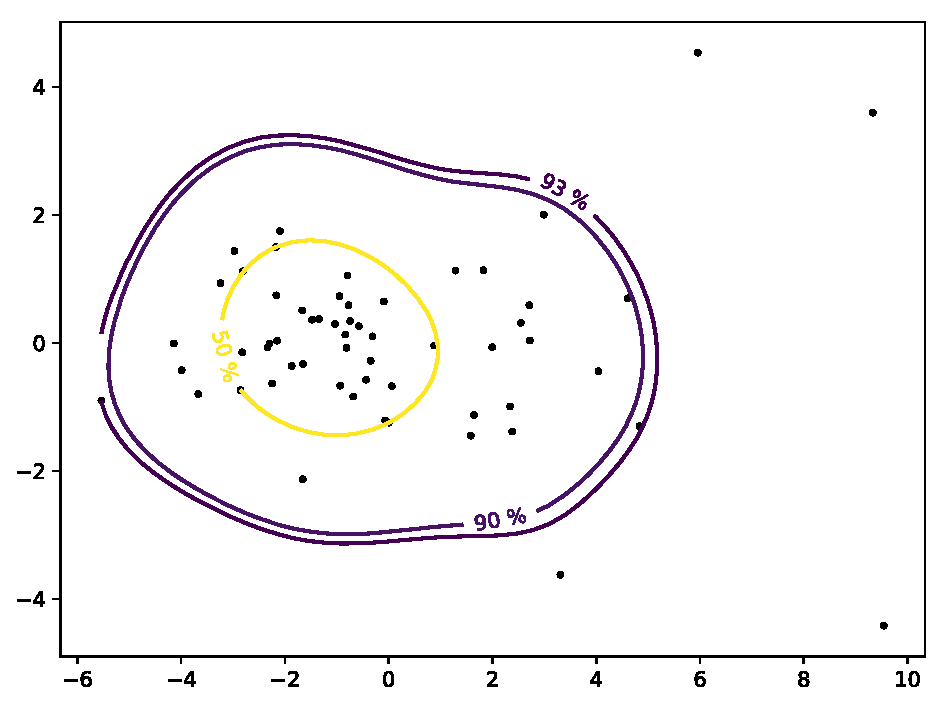
\includegraphics[width=0.45\linewidth,height=\textheight,keepaspectratio]{fig/contributions/visu/hdr_scatter.pdf}}
\subfloat[]{
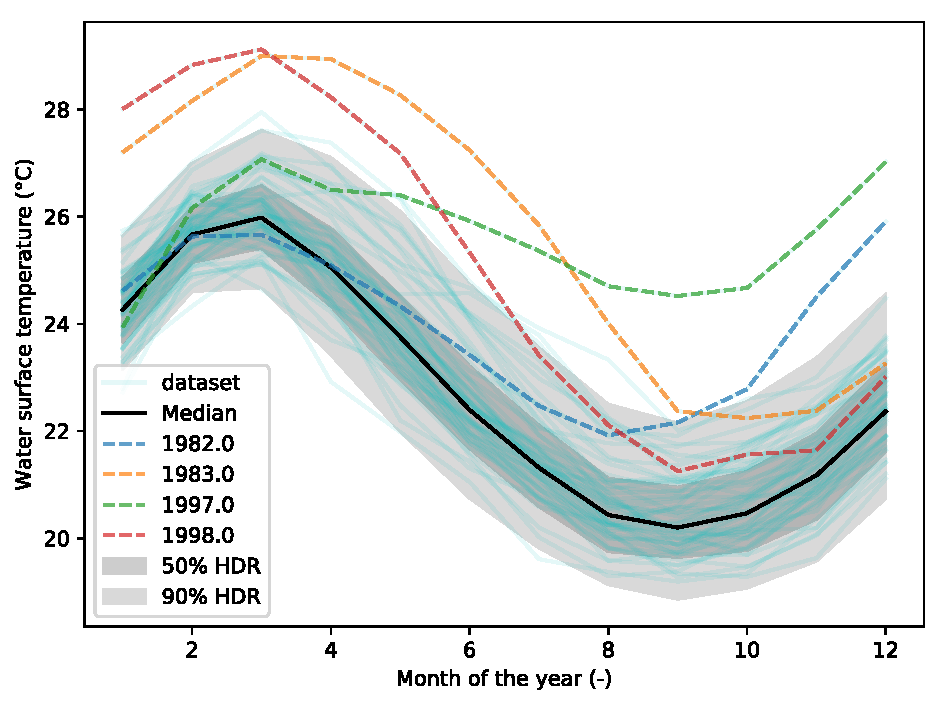
\includegraphics[width=0.45\linewidth,height=\textheight,keepaspectratio]{fig/contributions/visu/hdr_curves.pdf}} 
\caption{HDR boxplot on the El Ni\~no dataset. \textbf{a} scatter plot of the 2-dimensional reduced space with each dot as a realization. \textbf{b} dataset visualization with each curve as a realization from the database. Shaded areas are confidence intervals, \emph{thick solid black} line is the mean realization and \emph{highlighted-dashed} curves are outliers.}
\label{fig:elnino}
\end{figure*}

\cref{fig:elnino} illustrates the HDR boxplot for the El Ni\~no dataset in the reduced space (left panel) when only two modes are retained ensuring that at least 80\% of the response variable variance is conserved and in the output space (right) panel. Each realization is characterized with respect to the HDR metric. In the modal space, each dot represents a realization within the dataset and the contouring represents the 50\% and 90\% quantiles. In the response variable physical space, cyan curves represent the realizations from the dataset, the outliers are coloured-dashed curves, the thick black curve is the median and the grey shaded areas represent 50\% and 90\% quantiles envelopes. It should be noted that additional realizations with chosen characteristics on the outputs could be drawn by sampling the input for specific HDR criteria.


%\section{Software}\label{sec:software}



\chapter{Scientific Questions}\label{chap:questions}

\lettrine{F}{rom} this literature review, I propose through this thesis to contribute to three axis:

\begin{itemize}
\item \emph{How to construct a DoE in a high dimensional parameter space?}\hfill\\
	The number of simulation at hand is highly constrained by the computational power, the cost and the return time. A surrogate can only interpolate the physic which has already been seen, hence the need to explore uniformly the parameter space. When the number of parameters is high, controlling the sparsity in the DoE is challenging. I have developed a new sampling strategy that is versatile  and perform well with such constrains.
	
\item \emph{How to resample a DoE by considering the QoI of already sampled experiments?}\hfill\\
	Using the aforementioned novel method, it is possible to iteratively complet the DoE. This method does not incorporate any prior information on the shape of the response of the system. Here I propose a method which combine a Gaussian Process surrogate model with a LOOCV procedure in order to add a new sample in the DoE. This method has proven good behaviour in high dimensional parameter space.

\item \emph{How to visualize uncertainties in high dimensional cases?}\hfill\\
    Analysing both input parameter space and QoI is challenging when the dimension is high. I present some new ways to help understand uncertainties in this context.
\end{itemize}







